\documentclass[11pt]{article}
% Adapted from an original template by Hlyni Arnórssyni,
% Reykjavik University, Iceland

% ------------------------------ PAGE SETTINGS ------------------------------
\usepackage{geometry}

\geometry{
    paper=a4paper,
    top=2.5cm,
    bottom=2.5cm,
    left=2.5cm,
    right=2.4cm,
    headheight=0.75cm,
    footskip=1.5cm,
    headsep=0.75cm
}

% ------------------------------ BASIC PACKAGES ------------------------------
\usepackage{blindtext}

% Character encoding
\usepackage[T1]{fontenc}
\usepackage[utf8]{inputenc}

% Mathematics
\usepackage{amsmath, amsfonts, amsthm, amssymb}
\usepackage{braket, nicefrac}

% SI units
\usepackage{siunitx}

% Lists / columns
\usepackage{enumitem, multicol}

% ------------------------------ FIGURES ------------------------------
\usepackage{graphicx}
\usepackage{float}
\usepackage{keystroke}
\usepackage{pgfplots}
\usepgfplotslibrary{units}
\pgfplotsset{compat=1.16}

% Search these locations automatically for figures
\graphicspath{{fig/}{graphics/}{Graphics/}{./}}

% ------------------------------ TABLES ------------------------------
\usepackage{tabularx}
\usepackage{array}
\usepackage[table]{xcolor}

% ------------------------------ TYPOGRAPHY ------------------------------
\usepackage{caption}
\usepackage{titlesec}
\usepackage{microtype}
\usepackage{csquotes}

% ------------------------------ COLORS ------------------------------
\definecolor{GWBlue}{HTML}{1E4E79}

% ------------------------------ SECTION STYLING ------------------------------
\titleformat{\section}
  {\Large\bfseries\color{GWBlue}}
  {\thesection.}
  {0.40em}
  {}

\titlespacing*{\section}
  {0pt}
  {0.70em}
  {0.28em}

% ------------------------------ CAPTION STYLING ------------------------------
\captionsetup{
    font=small,
    labelfont=bf,
    textfont=it,
    labelsep=period,
    skip=4pt
}

% ------------------------------ PARAGRAPH SPACING ------------------------------
\setlength{\parindent}{0pt}
\setlength{\parskip}{0.30em}

% ------------------------------ BIBLIOGRAPHY ------------------------------
\usepackage[
    backend=biber,
    style=authoryear,
    sorting=none,
    giveninits=true,
    maxbibnames=99,
    dashed=false
]{biblatex}

\addbibresource{references.bib}

\DeclareNameAlias{sortname}{family-given}
\DeclareNameAlias{default}{family-given}
\DeclareFieldFormat[article]{title}{#1}
\DeclareFieldFormat[misc]{title}{#1}
\renewbibmacro{in:}{}

\AtEveryBibitem{%
    \clearfield{doi}%
    \clearfield{urldate}%
}

\AtBeginBibliography{\small}
\setlength{\bibitemsep}{0.35em}

% ------------------------------ HYPERLINKS ------------------------------
\usepackage{hyperref}

\hypersetup{
    colorlinks=true,
    linkcolor=GWBlue,
    citecolor=GWBlue,
    urlcolor=GWBlue
}
\newcolumntype{C}[1]{>{\centering\arraybackslash}p{#1}}
\setlength{\emergencystretch}{3em}
\graphicspath{{fig/}{fig/hard_example_mining/curriculum_comparison/}{fig/targeted_augmentation/augmentation_comparison/}{fig/som_reanalysis/}}
\usetikzlibrary{positioning,arrows.meta}
\begin{document}

\begin{titlepage}
\centering
\thispagestyle{empty}
\vspace*{0.15in}

\includegraphics[width=0.5\textwidth]{gwu_logo.pdf}
\vspace{0.28in}

{\large\bfseries Data Science Program\par}
{\large\bfseries Department of Data Science\par}
{\large DATS 6501 - Capstone Project - Fall 2026\par}
\vspace{0.38in}
{\Large\bfseries Post-Training Analysis \& Novelty Detection Using\par}
\vspace{0.08in}
{\Large\bfseries Neural Network Self-Organizing Maps (NNSOM)\par}
\vspace{0.34in}
{\large\bfseries PHASE 4 REPORT\par}
\vspace{0.22in}
{\large\bfseries Guided Retraining\par}
\vspace{0.12in}
{\large\bfseries Fashion-MNIST\par}
\vspace{0.36in}
{\large\bfseries Capstone - Group 5\par}
\vspace{0.08in}
{\large\bfseries Fyrooz Anika Khan\par}
{\large\bfseries Nazish Atta\par}
\vspace{0.30in}
{\large The George Washington University\par}
{\large Washington, DC\par}
\vspace{0.30in}
{\large\itshape Supervised by\par}
{\large\itshape Dr. Amir Jafari\par}
{\large\itshape Associate Professor of Data Science\par}
\vspace*{\fill}
\end{titlepage}

\section{Summary}

Phase 4 asks one question: \emph{can the SOM help us train a better CNN?} The SOM is a map that shows where the CNN makes its mistakes. We used it to pick the ``hard'' training images and then retrained the CNN (LeNet-5, on Fashion-MNIST clothing images \parencite{xiao2017fashion}) in two ways: \textbf{curriculum learning} (the hard images are let in slowly) and \textbf{targeted augmentation} (we add slightly changed copies of the hard images). Every idea was compared with a fair control that uses the same number of images, repeated 5 times, and checked once on the test images. Last, we trained new SOMs on the retrained CNNs to see whether the map itself changed, and tested whether the new maps still detect novel images. The design is the MNIST Phase 4 design, copied unchanged except where Fashion-MNIST made that impossible (Section~\ref{sec:deviation}).

\begin{itemize}[leftmargin=1.4em, itemsep=1pt]
  \item \textbf{Targeted augmentation did not clearly help.} On the SOM's error regions (the ``hotspots''), mistakes fell from 36.0\% to 34.0\% with SOM-chosen images and to 35.0\% with random ones, but neither difference is clear. The primary statement (SOM-chosen beats random on the hotspots) is \textbf{not met}. On MNIST it was met.
  \item \textbf{Overall accuracy did not change.} Every augmentation arm stays at 90.5--90.7\% test accuracy (normal training: 90.66\%).
  \item \textbf{Curriculum learning hurt, more than on MNIST.} It lowered test accuracy to 87.37\% (SOM-chosen order) and 89.15\% (random order), against 90.66\% for normal training.
  \item \textbf{The new SOMs are not cleaner.} After SOM-guided augmentation, the weak regions of a new map hold fewer mistakes than after random augmentation (40.5\% against 43.7\%), but not fewer than after normal training (40.6\%), and the neurons are not purer (Section~\ref{sec:reanalysis}).
  \item \textbf{The SOM still detects novel images after retraining, but less well.} Every retrained network's SOM separates SVHN from Fashion-MNIST better than chance (AUROC 0.59 to 0.93), but SOM-guided retraining \emph{lowered} the SOM's AUROC compared with normal training (0.715 against 0.838; Section~\ref{sec:novelty_after}). On MNIST, retraining left it unchanged.
\end{itemize}

\subsection*{Where each item of the plan is covered}

{\small
\renewcommand{\arraystretch}{1.12}
\begin{tabularx}{\textwidth}{|>{\raggedright\arraybackslash}p{0.50\textwidth}|X|}
\hline
\textbf{What Phase 4 asks for} & \textbf{Where} \\ \hline
Hard-example pool and curriculum against standard training & Section~\ref{sec:method}, Tables~\ref{tab:pools}--\ref{tab:criteria}, Figures~\ref{fig:cf_cur} and~\ref{fig:curves} \\ \hline
Targeted augmentation and its effect on the rest of the data & Tables~\ref{tab:arms}--\ref{tab:criteria}, Figures~\ref{fig:cf_aug} and~\ref{fig:curves}, Appendix \\ \hline
Re-extract features, re-train the SOM, compare old and new maps & Section~\ref{sec:reanalysis}, Table~\ref{tab:reanalysis}, Figures~\ref{fig:reanalysis_measures}--\ref{fig:reanalysis_purity} \\ \hline
Feedback loop: SOM analysis $\rightarrow$ retraining $\rightarrow$ new SOM structure & Figure~\ref{fig:loop}, Section~\ref{sec:meaning} \\ \hline
Table: baseline accuracy, post-retraining accuracy & Tables~\ref{tab:arms} and~\ref{tab:vs_standard} \\ \hline
Table: novelty detection AUROC after retraining & Section~\ref{sec:novelty_after}, Table~\ref{tab:novelty_after} \\ \hline
Monitor forgetting of easy examples & Section~\ref{sec:meaning} (last item), Figure~\ref{fig:curves} \\ \hline
Before/after comparison and learning curves & Figures~\ref{fig:cf_aug}--\ref{fig:curves} \\ \hline
Comparison with MNIST & Table~\ref{tab:mnist} \\ \hline
\end{tabularx}}

\section{Key terms in plain words}

\renewcommand{\arraystretch}{1.12}
{\small
\begin{tabularx}{\textwidth}{|>{\raggedright\arraybackslash}p{0.22\textwidth}|X|}
\hline
\textbf{Term} & \textbf{What it means} \\ \hline
CNN, LeNet-5 & The neural network that looks at a picture of a clothing item and says which of the 10 classes it is (T-shirt/top, Trouser, Pullover, Dress, Coat, Sandal, Shirt, Sneaker, Bag, Ankle boot). \\ \hline
SOM & A ``map'' that places similar images close together. We train it on what the CNN has learned, so we can see where the CNN gets confused. \\ \hline
Neuron, purity & A neuron is one cell of the map. Its purity is how many of its images show the same class; low purity means a mixed, confusing cell. \\ \hline
Hotspot & A map cell where the CNN makes many mistakes (11 cells in our map). \\ \hline
Hard image, pool & A training image that sits in a hotspot, in a mixed cell, or far from its cell. All hard images together are the \emph{pool} (19{,}997 images). \\ \hline
Curriculum learning & Teach like school: start with easy images and let the hard ones in step by step. \\ \hline
Augmentation & Adding copies of an image that are slightly changed (turned, shifted, zoomed, sheared) so the CNN sees more variety. \\ \hline
Control & A fair comparison that uses the same number of added images but picks them differently: \emph{random} (by chance, same class mix) or \emph{msp} (the images the CNN is least sure about). \\ \hline
Max-softmax (MSP) & The CNN's confidence in its answer. Low confidence means ``not sure''. \\ \hline
Seed & A number that fixes the randomness of one training run. We repeat every experiment with 5 seeds so one lucky run does not fool us. \\ \hline
Validation / test images & Validation images are used while building and checking the method. Test images are kept untouched and used once at the end, like an exam. \\ \hline
Error, accuracy & Error is the share of images the CNN gets wrong; accuracy is the share it gets right. \\ \hline
Confusion matrix (CF1, CF2) & A table of true class against predicted class; the diagonal is correct answers, everything else is mistakes. CF1 is before retraining (normal training), CF2 is after. \\ \hline
95\% interval & The range in which the true difference very likely lies. If it does not include 0, the difference is probably real and not luck. \\ \hline
Paired difference & Two methods compared seed by seed (the same seed for both), so that the comparison is fair. \\ \hline
Macro-F1 guard & A safety check that the CNN did not get worse on some classes while improving on others. \\ \hline
Transform check & A test, before any training, that the altered copies are still recognisable: the Phase 1 network may lose at most 2 points of validation accuracy on them. \\ \hline
Forgetting & The CNN becoming worse on images it already handled well after being retrained. \\ \hline
Weighted purity & The share of images that show the main class of their neuron. Higher means cleaner class regions. \\ \hline
Class scatter index & How many separate patches of the map one class occupies on average. 1 means every class has one connected region. \\ \hline
Topographic error & The share of images whose two closest neurons are not neighbours on the map. Lower means a better ordered map. \\ \hline
CKA & A score from 0 to 1 for how similar the embeddings of two networks are; 1 means the same. \\ \hline
\end{tabularx}}

\section{Method}\label{sec:method}

The loop is: SOM analysis $\rightarrow$ targeted retraining $\rightarrow$ re-analysis (Figure~\ref{fig:loop}). The retraining algorithm is fixed in advance and is the same for every arm. All rules are those of the MNIST Phase 4 protocol; the Fashion-MNIST protocol (\texttt{RETRAINING\_PROTOCOL.md}) copies them and was stamped (SHA-256 of the protocol and the configuration) on 2026-11-22 at 07:17 UTC, before the test split was read.

\begin{figure}[H]
\centering
\begin{tikzpicture}[
  font=\footnotesize, node distance=9mm,
  box/.style={draw=GWBlue, rounded corners=2pt, align=center, minimum height=13mm, minimum width=42mm, fill=GWBlue!6, line width=0.6pt},
  arr/.style={-{Stealth[length=2mm]}, line width=0.7pt, draw=GWBlue}]
\node[box] (a) {\textbf{1. SOM analysis}\\ 11 hotspot neurons,\\ 19{,}997 hard training images};
\node[box, right=of a] (b) {\textbf{2. Targeted retraining}\\ curriculum or\\ augmented copies};
\node[box, right=of b] (c) {\textbf{3. New SOMs}\\ trained on the retrained\\ CNNs, 15 maps};
\draw[arr] (a)--(b); \draw[arr] (b)--(c);
\draw[arr, dashed] (c.south) -- ++(0,-6mm) -| (a.south);
\end{tikzpicture}
\caption{The feedback loop of Phase 4. The dashed arrow marks the next round, which this report does not run.}
\label{fig:loop}
\end{figure}

\begin{enumerate}[leftmargin=1.6em, itemsep=1pt]
  \item \textbf{Select hard images (training images only, true labels).} A training image is in the \emph{SOM pool} if its neuron is one of the 11 error hotspots of the Phase 2 map, or its neuron's purity is below 0.95, or its distance to its neuron is above the 95th percentile. A smaller \emph{hotspot pool} uses the first rule only. Table~\ref{tab:pools} gives the sizes.
  \item \textbf{Build controls of the same size.} \emph{random}: random images with the same class mix, redrawn for each seed. \emph{msp}: the images with the lowest max-softmax confidence. \emph{standard}: nothing added.
  \item \textbf{Retrain from scratch, once per arm.} LeNet-5 \parencite{lecun1998gradient} with the Phase 1 recipe (Adam \parencite{kingma2015adam}, 20 epochs), seeds 1 to 5, the same seeds for all arms.
  \begin{itemize}[leftmargin=1.2em, itemsep=0pt]
    \item \emph{Curriculum:} all easy images plus 10\% of the hard pool, with 10\% more every 5 epochs (easiest first), so the last epochs use 40\% of the pool.
    \item \emph{Augmentation:} all original images plus 3 altered copies of every pool image (rotation up to 2.5$^\circ$, shift up to 0.25 pixel, zoom 0.975 to 1.025, shear up to 2$^\circ$, no flips; revision r3, Section~\ref{sec:deviation}). Two \emph{paced} arms add the same copies gradually, as in the curriculum.
  \end{itemize}
  \item \textbf{Evaluate once on the test split (10{,}500 images, 422 of them on hotspot neurons).} CF1 is the confusion matrix of the \texttt{standard} arm, CF2 that of a retrained arm. Differences between arms are paired bootstrap intervals over the test images (2{,}000 resamples, seed 2026), computed on the mean of the 5 seeds.
\end{enumerate}

\begin{table}[H]
\centering
\renewcommand{\arraystretch}{1.1}
\small
\begin{tabular}{|l|C{0.11\textwidth}|C{0.13\textwidth}|C{0.17\textwidth}|}
\hline
\textbf{Pool (training images)} & \textbf{Images} & \textbf{Share of 49,000} & \textbf{Training errors inside} \\ \hline
On a hotspot neuron (hotspot pool) & 1,909 & 3.9\% & 521 \\ \hline
In a neuron with purity $<0.95$ & 18,537 & 37.8\% & 3,071 \\ \hline
Distance to neuron above the 95th percentile & 2,450 & 5.0\% & 164 \\ \hline
\textbf{SOM pool} (any of the three) & \textbf{19,997} & \textbf{40.8\%} & \textbf{3,092} \\ \hline
msp pool (same size) & 19,997 & 40.8\% & 3,264 \\ \hline
In both the SOM and the msp pool & 16,213 & 33.1\% & 3,077 \\ \hline
\end{tabular}
\caption{The hard-image pools. The Phase 1 network makes 3,311 mistakes on the training images; 3,092 of them are in the SOM pool. MNIST's SOM pool held 4,217 images (8.6\%). By class, the SOM pool is mostly upper-body clothing: Coat 4,331, Shirt 3,917, Pullover 3,325 and T-shirt/top 2,746 of 4,900 images each, against 226 Trousers. Source: \texttt{hard\_example\_pools\_som\_15x15\_nb11\_ep250\_s42/tables/}.}
\label{tab:pools}
\end{table}

\textbf{Success criteria} (written down before the test split was used): C1, curriculum\_som has lower overall error than standard; C2, curriculum\_som has lower hotspot error than curriculum\_random; A1 (primary), augmented\_som has lower hotspot error than augmented\_random; A2, augmented\_som has lower hotspot error than standard; A3, augmented\_som does not raise the error outside the hotspots by more than 0.2 points. C1, C2, A1 and A2 also need an interval that excludes 0 and a macro-F1 that does not fall by more than 0.0033. That guard is twice the seed-to-seed standard deviation of the \texttt{standard} arm's validation macro-F1, the MNIST rule; it was measured on validation images before any arms were compared (MNIST: 0.0016).

\subsection*{Re-analysis with new SOMs}

The last step of the loop retrains nothing. For the \texttt{standard}, \texttt{augmented\_som} and \texttt{augmented\_random} arms and each of the 5 CNN seeds, we took the 84-dimensional embeddings of the training and validation images, trained a new 15$\times$15 SOM with the Phase 2 recipe (neighbourhood 11, 250 epochs, seed 42), and measured it on the validation split only; the test split was not read. That gives 15 new SOMs, plus the Phase 2 map as a read-only reference. The measures are weighted purity, the share of images in low-purity neurons ($<0.95$), a class scatter index, topographic error, the error rate on the 11 worst neurons (hotspots, picked by the lower Wilson bound of their error rate), the share of all errors that fall on those neurons, overall error, and linear CKA \parencite{kornblith2019cka} between networks. The first four follow the SOM quality measures surveyed by \textcite{forest2020somsurvey}; the class scatter index is our own implementation of their verbal description. Differences between arms are taken per seed, since the arms share seeds \parencite{bouthillier2021variance}, then averaged, with a 95\% $t$-interval over the 5 differences. The five statements below and the tolerance of 1.0 percentage point in R5 are the MNIST ones, unchanged.

\begin{itemize}[leftmargin=1.4em, itemsep=1pt]
  \item R1: purity is higher for \texttt{augmented\_som} than for \texttt{standard} (interval above 0).
  \item R2: hotspot error rate is lower for \texttt{augmented\_som} than for \texttt{standard} (interval below 0).
  \item R3: purity is higher for \texttt{augmented\_som} than for \texttt{augmented\_random}.
  \item R4: hotspot error rate is lower for \texttt{augmented\_som} than for \texttt{augmented\_random}.
  \item R5: topographic error of \texttt{augmented\_som} is not more than 1.0 point above \texttt{standard} (upper end of the interval at most 1.0).
\end{itemize}

\section{Results of the retraining}

Table~\ref{tab:arms} gives baseline and post-retraining accuracy; Table~\ref{tab:criteria} gives the verdicts. Figures~\ref{fig:cf_aug} and~\ref{fig:cf_cur} show CF1 and CF2 (the other arms are in the Appendix), and Figure~\ref{fig:curves} the learning curves. For reference, the single Phase 1 network (seed 42) scored 90.90\% on the test split.

\begin{table}[H]
\centering
\renewcommand{\arraystretch}{1.1}
\small
\begin{tabular}{|l|C{0.20\textwidth}|C{0.20\textwidth}|C{0.20\textwidth}|}
\hline
\textbf{Arm} & \textbf{Test accuracy (\%)} & \textbf{Hotspot error (\%)} & \textbf{Non-hotspot error (\%)} \\ \hline
\textbf{standard} (baseline, CF1) & 90.66 (0.23) & 36.0 (1.7) & 8.22 (0.18) \\ \hline
\multicolumn{4}{|l|}{\textit{Curriculum}} \\ \hline
curriculum\_som & 87.37 (0.19) & 51.8 (2.1) & 10.99 (0.23) \\ \hline
curriculum\_random & 89.15 (0.29) & 42.1 (1.5) & 9.54 (0.25) \\ \hline
curriculum\_msp & 87.07 (0.27) & 50.0 (1.9) & 11.38 (0.26) \\ \hline
\multicolumn{4}{|l|}{\textit{Targeted augmentation}} \\ \hline
augmented\_som & 90.62 (0.42) & 34.0 (2.3) & 8.35 (0.42) \\ \hline
augmented\_random & 90.60 (0.26) & 35.0 (2.8) & 8.33 (0.16) \\ \hline
augmented\_msp & 90.57 (0.34) & 35.2 (1.4) & 8.35 (0.30) \\ \hline
augmented\_hotspot & 90.52 (0.25) & 36.4 (2.1) & 8.35 (0.22) \\ \hline
augmented\_random\_hotspot & 90.53 (0.22) & 36.6 (1.4) & 8.34 (0.18) \\ \hline
augmented\_som\_paced & 90.65 (0.14) & 35.0 (0.8) & 8.28 (0.12) \\ \hline
augmented\_random\_paced & 90.60 (0.20) & 36.5 (1.7) & 8.27 (0.16) \\ \hline
\end{tabular}
\caption{Test results, mean (standard deviation) over 5 seeds. Hotspot error is measured on the 422 test images that fall on hotspot neurons, non-hotspot error on the other 10,078. Both experiments use the same \texttt{standard} arm. Source: \texttt{tables/test\_summary.csv} of the two comparison runs.}
\label{tab:arms}
\end{table}

\begin{table}[H]
\centering
\renewcommand{\arraystretch}{1.12}
\small
{\setlength{\tabcolsep}{3pt}\begin{tabular}{|C{0.06\textwidth}|>{\raggedright\arraybackslash}p{0.38\textwidth}|C{0.22\textwidth}|C{0.14\textwidth}|C{0.10\textwidth}|}
\hline
\textbf{ID} & \textbf{Comparison (error on)} & \textbf{Difference in points [95\% CI]} & \textbf{Macro-F1 guard} & \textbf{Verdict} \\ \hline
C1 & curriculum\_som $-$ standard (all test images) & +3.29 [+2.93, +3.64] & $-$0.0343 (fails) & \textbf{not met} \\ \hline
C2 & curriculum\_som $-$ curriculum\_random (hotspots) & +9.76 [+6.64, +12.84] & $-$0.0183 (fails) & \textbf{not met} \\ \hline
A1 & augmented\_som $-$ augmented\_random (hotspots) & $-$1.04 [$-$3.22, +1.14] & +0.0003 (holds) & \textbf{not met} \\ \hline
A2 & augmented\_som $-$ standard (hotspots) & $-$1.99 [$-$4.79, +0.71] & $-$0.0001 (holds) & \textbf{not met} \\ \hline
A3 & augmented\_som $-$ standard (non-hotspot images; limit: upper end $\le 0.2$) & +0.13 [$-$0.12, +0.37] &  & \textbf{not met} \\ \hline
\multicolumn{5}{|l|}{\textit{Also reported (not success criteria)}} \\ \hline
E1 & augmented\_som $-$ augmented\_msp (hotspots) & $-$1.23 [$-$3.27, +0.81] &  & \textbf{tie} \\ \hline
E2 & augmented\_som\_paced $-$ augmented\_som (hotspots) & +1.04 [$-$1.52, +3.60] &  & \textbf{tie} \\ \hline
E3 & augmented\_hotspot $-$ augmented\_random\_hotspot (hotspots) & $-$0.28 [$-$2.27, +1.71] &  & \textbf{tie} \\ \hline
\end{tabular}}
\caption{The success criteria, fixed before the test split was used. Negative differences mean fewer errors for the first arm; 1 test hotspot image is about 0.24 points. Intervals: paired bootstrap over test images, mean of 5 seeds. The macro-F1 guard is the first arm's macro-F1 minus the second arm's; it may not fall below $-0.0033$. A3 fails because the upper end (0.37) is above 0.2, not because the error clearly rose. E1 to E3 are the extra comparisons the MNIST report calls R1 to R3. Source: \texttt{test\_results.json} of the two comparison runs.}
\label{tab:criteria}
\end{table}

\textbf{Every arm against normal training.} The protocol also asks for every arm compared with \texttt{standard} (Table~\ref{tab:vs_standard}; not success criteria). No augmentation arm differs clearly from \texttt{standard} on any subset: all 21 intervals include 0. The two paced arms cannot be told apart on the hotspots ($-1.47$ points, $-3.32$ to $+0.38$), and pacing makes no clear difference against the unpaced twins. All three curriculum orders are clearly worse than \texttt{standard}, the random order included (+1.51 points overall), unlike on MNIST, where only the SOM and least-confident orders were. The SOM order is slightly better than the least-confident order on overall error ($-0.30$ points, $-0.60$ to $-0.01$), but not on the hotspots.

\begin{table}[H]
\centering
\renewcommand{\arraystretch}{1.1}
\footnotesize
{\setlength{\tabcolsep}{4pt}\begin{tabular}{|l|C{0.22\textwidth}|C{0.22\textwidth}|C{0.22\textwidth}|}
\hline
\textbf{Arm $-$ standard} & \textbf{All test images} & \textbf{Hotspot images} & \textbf{Non-hotspot images} \\ \hline
augmented\_som & +0.04 [$-$0.22, +0.30] & $-$1.99 [$-$4.79, +0.71] & +0.13 [$-$0.12, +0.37] \\ \hline
augmented\_random & +0.06 [$-$0.17, +0.31] & $-$0.95 [$-$3.36, +1.33] & +0.11 [$-$0.12, +0.35] \\ \hline
augmented\_msp & +0.09 [$-$0.15, +0.35] & $-$0.76 [$-$3.27, +1.66] & +0.13 [$-$0.10, +0.36] \\ \hline
augmented\_hotspot & +0.14 [$-$0.08, +0.35] & +0.38 [$-$1.80, +2.51] & +0.13 [$-$0.08, +0.32] \\ \hline
augmented\_random\_hotspot & +0.13 [$-$0.06, +0.32] & +0.66 [$-$1.09, +2.47] & +0.11 [$-$0.06, +0.28] \\ \hline
augmented\_som\_paced & +0.01 [$-$0.17, +0.21] & $-$0.95 [$-$2.75, +0.95] & +0.05 [$-$0.13, +0.24] \\ \hline
augmented\_random\_paced & +0.06 [$-$0.13, +0.26] & +0.52 [$-$1.47, +2.42] & +0.04 [$-$0.12, +0.22] \\ \hline
curriculum\_som & \textbf{+3.29 [+2.93, +3.64]} & \textbf{+15.88 [+12.04, +19.62]} & \textbf{+2.76 [+2.44, +3.08]} \\ \hline
curriculum\_random & \textbf{+1.51 [+1.25, +1.77]} & \textbf{+6.11 [+3.55, +8.63]} & \textbf{+1.32 [+1.08, +1.55]} \\ \hline
curriculum\_msp & \textbf{+3.59 [+3.24, +3.96]} & \textbf{+14.03 [+10.33, +17.58]} & \textbf{+3.15 [+2.79, +3.49]} \\ \hline
\end{tabular}}
\caption{Every arm minus \texttt{standard}: difference in test error, percentage points, with the 95\% paired bootstrap interval over test images (mean of 5 seeds). Bold: the interval excludes 0. Also reported, not success criteria. Source: \texttt{tables/test\_comparisons.csv} of the two comparison runs.}
\label{tab:vs_standard}
\end{table}

\textbf{Validation results.} The validation split was used before the test pass, for the checks only: the macro-F1 guard is twice the standard deviation of the \texttt{standard} row's macro-F1 ($2\times0.0017=0.0033$). Table~\ref{tab:validation} gives every arm on it, for completeness; no arm, threshold or setting was chosen from it. As on the test split, the augmentation arms stay within about 0.3 points of \texttt{standard} overall, \texttt{augmented\_som} has the lowest hotspot error, and all three curricula are clearly worse.

\begin{table}[H]
\centering
\renewcommand{\arraystretch}{1.1}
\footnotesize
\begin{tabular}{|l|C{0.18\textwidth}|C{0.18\textwidth}|C{0.18\textwidth}|}
\hline
\textbf{Arm} & \textbf{Validation error (\%)} & \textbf{Hotspot error (\%)} & \textbf{Macro-F1} \\ \hline
standard & 8.65 (0.15) & 37.6 (2.0) & 0.9133 (0.0017) \\ \hline
\multicolumn{4}{|l|}{\textit{Curriculum}} \\ \hline
curriculum\_som & 11.95 (0.27) & 51.7 (1.6) & 0.8788 (0.0025) \\ \hline
curriculum\_random & 10.67 (0.26) & 44.6 (1.6) & 0.8921 (0.0023) \\ \hline
curriculum\_msp & 12.11 (0.21) & 49.9 (1.4) & 0.8763 (0.0029) \\ \hline
\multicolumn{4}{|l|}{\textit{Targeted augmentation}} \\ \hline
augmented\_som & 8.67 (0.19) & 35.8 (2.3) & 0.9133 (0.0019) \\ \hline
augmented\_random & 8.78 (0.10) & 37.3 (1.0) & 0.9122 (0.0009) \\ \hline
augmented\_msp & 8.73 (0.24) & 36.7 (3.3) & 0.9125 (0.0023) \\ \hline
augmented\_hotspot & 8.79 (0.11) & 36.3 (1.4) & 0.9119 (0.0012) \\ \hline
augmented\_random\_hotspot & 8.91 (0.15) & 38.5 (3.0) & 0.9108 (0.0015) \\ \hline
augmented\_som\_paced & 8.71 (0.06) & 38.1 (1.2) & 0.9126 (0.0007) \\ \hline
augmented\_random\_paced & 8.75 (0.18) & 37.7 (1.0) & 0.9123 (0.0019) \\ \hline
\end{tabular}
\caption{Validation results, mean (standard deviation) over 5 seeds, on the 10,500 validation images; hotspot error is on the validation images that fall on the 11 hotspot neurons. Source: \texttt{tables/validation\_summary.csv} of the two comparison runs.}
\label{tab:validation}
\end{table}

\begin{figure}[H]
\centering
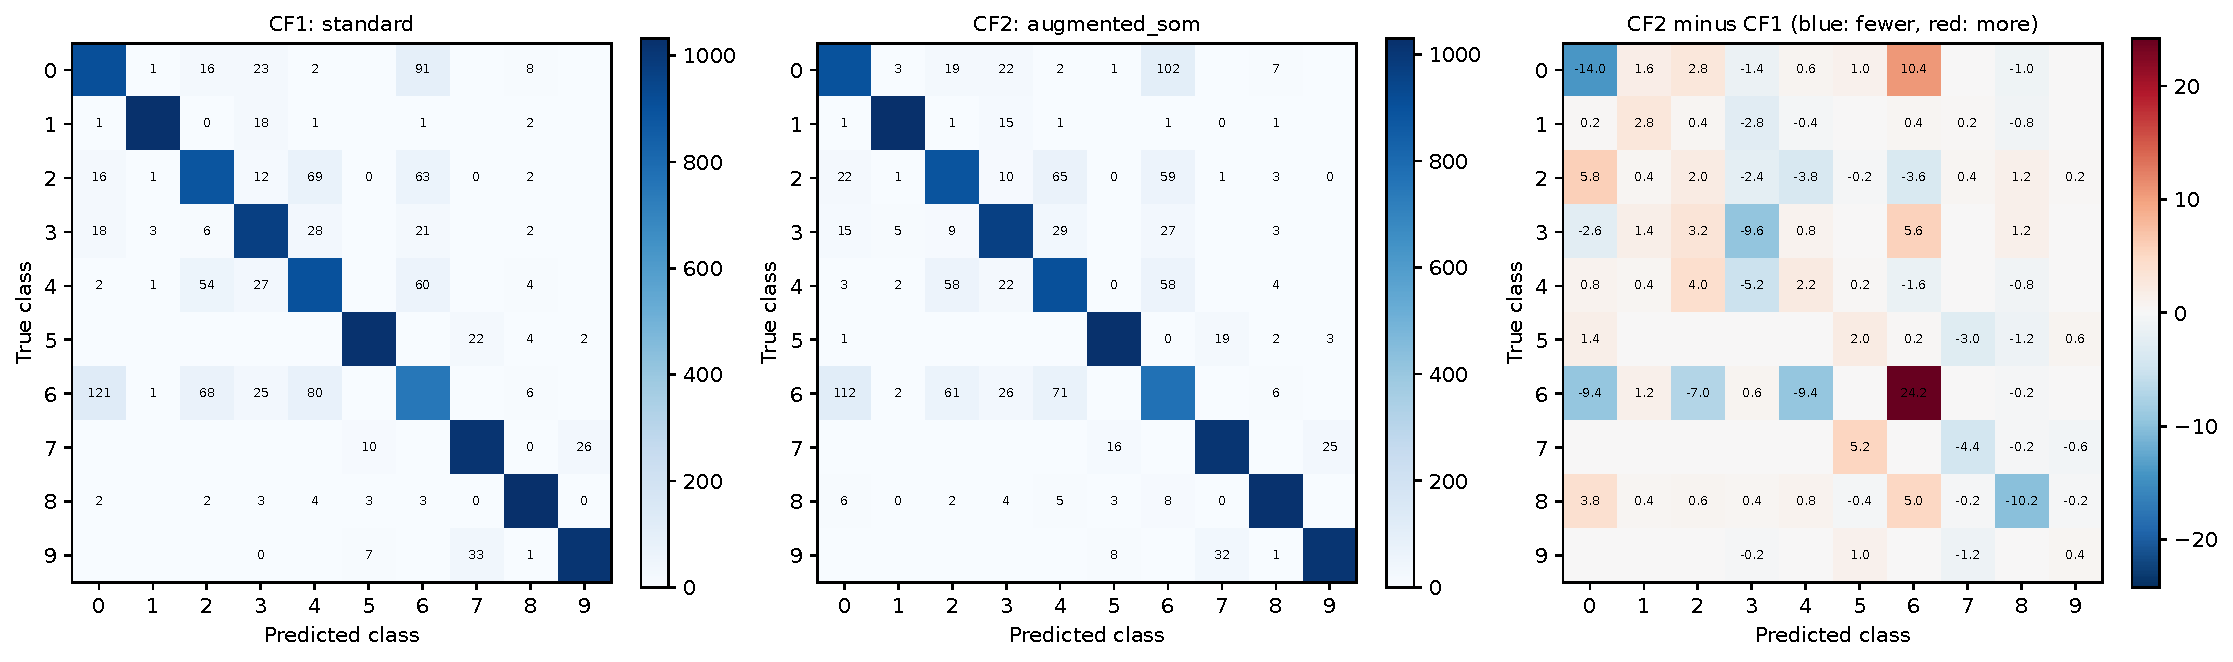
\includegraphics[width=\textwidth]{fig/targeted_augmentation/augmentation_comparison/confusion_standard_vs_augmented_som.pdf}
\caption{CF1 (standard) and CF2 (augmented\_som): mean test confusion matrices over 5 seeds, and their difference (blue: fewer cases, red: more). Classes: 0 T-shirt/top, 1 Trouser, 2 Pullover, 3 Dress, 4 Coat, 5 Sandal, 6 Shirt, 7 Sneaker, 8 Bag, 9 Ankle boot. The largest changes are on the diagonal of class 6 (more Shirts right) and class 0 (fewer T-shirts right), with Shirts now taken for T-shirts less often and T-shirts taken for Shirts more often.}
\label{fig:cf_aug}
\end{figure}

\begin{figure}[H]
\centering
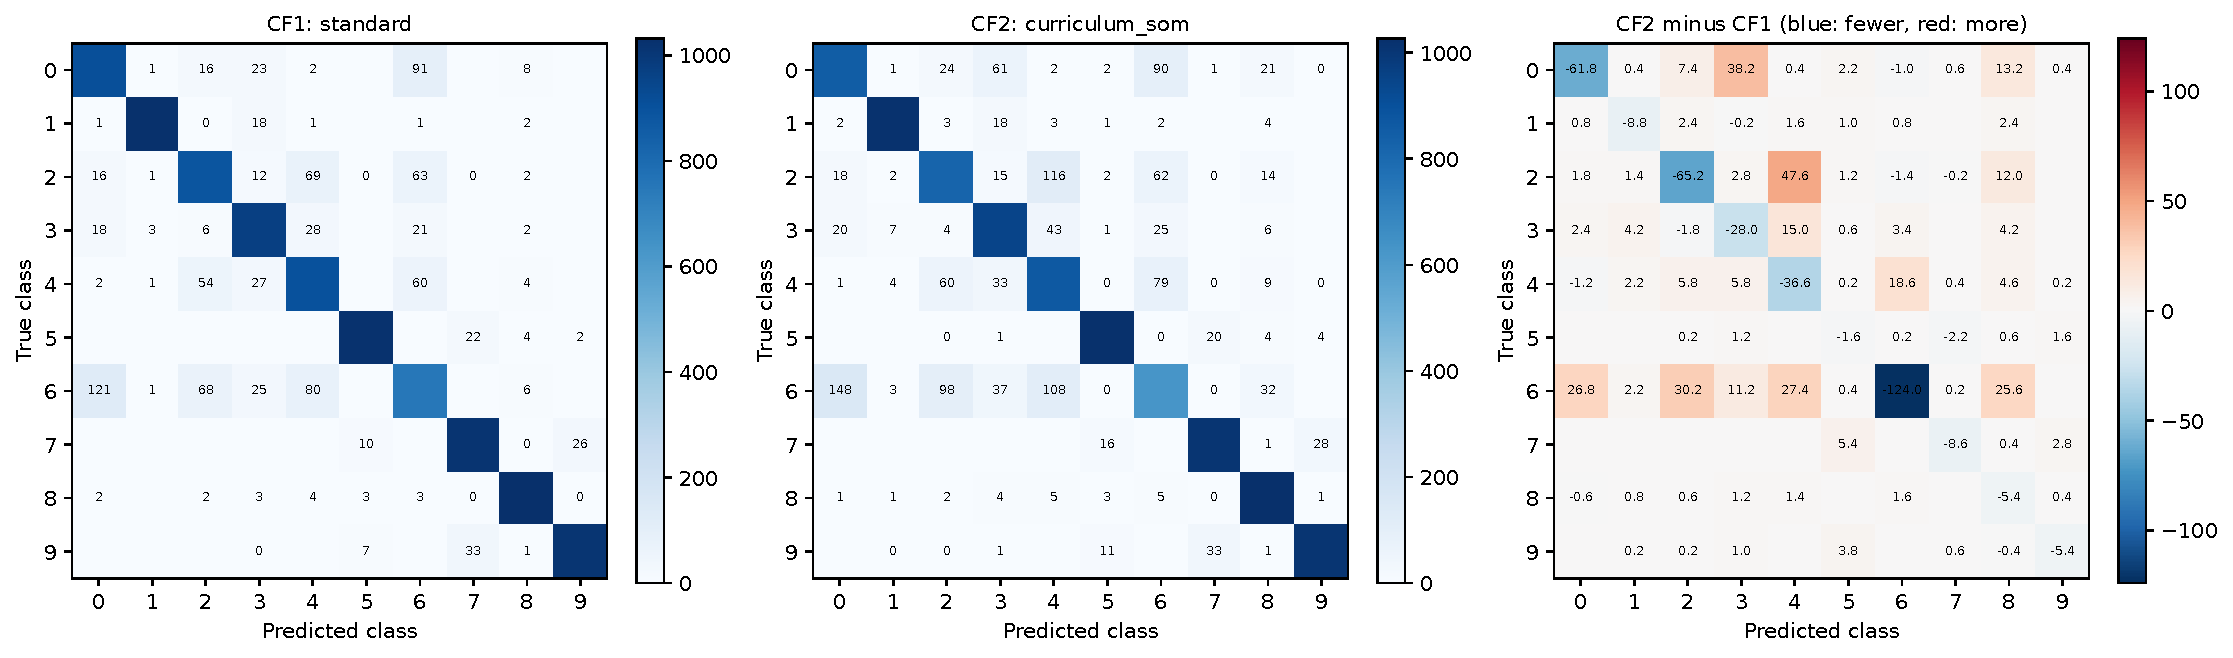
\includegraphics[width=\textwidth]{fig/hard_example_mining/curriculum_comparison/confusion_standard_vs_curriculum_som.pdf}
\caption{CF1 (standard) and CF2 (curriculum\_som), as in Figure~\ref{fig:cf_aug}.}
\label{fig:cf_cur}
\end{figure}

\begin{figure}[H]
\centering
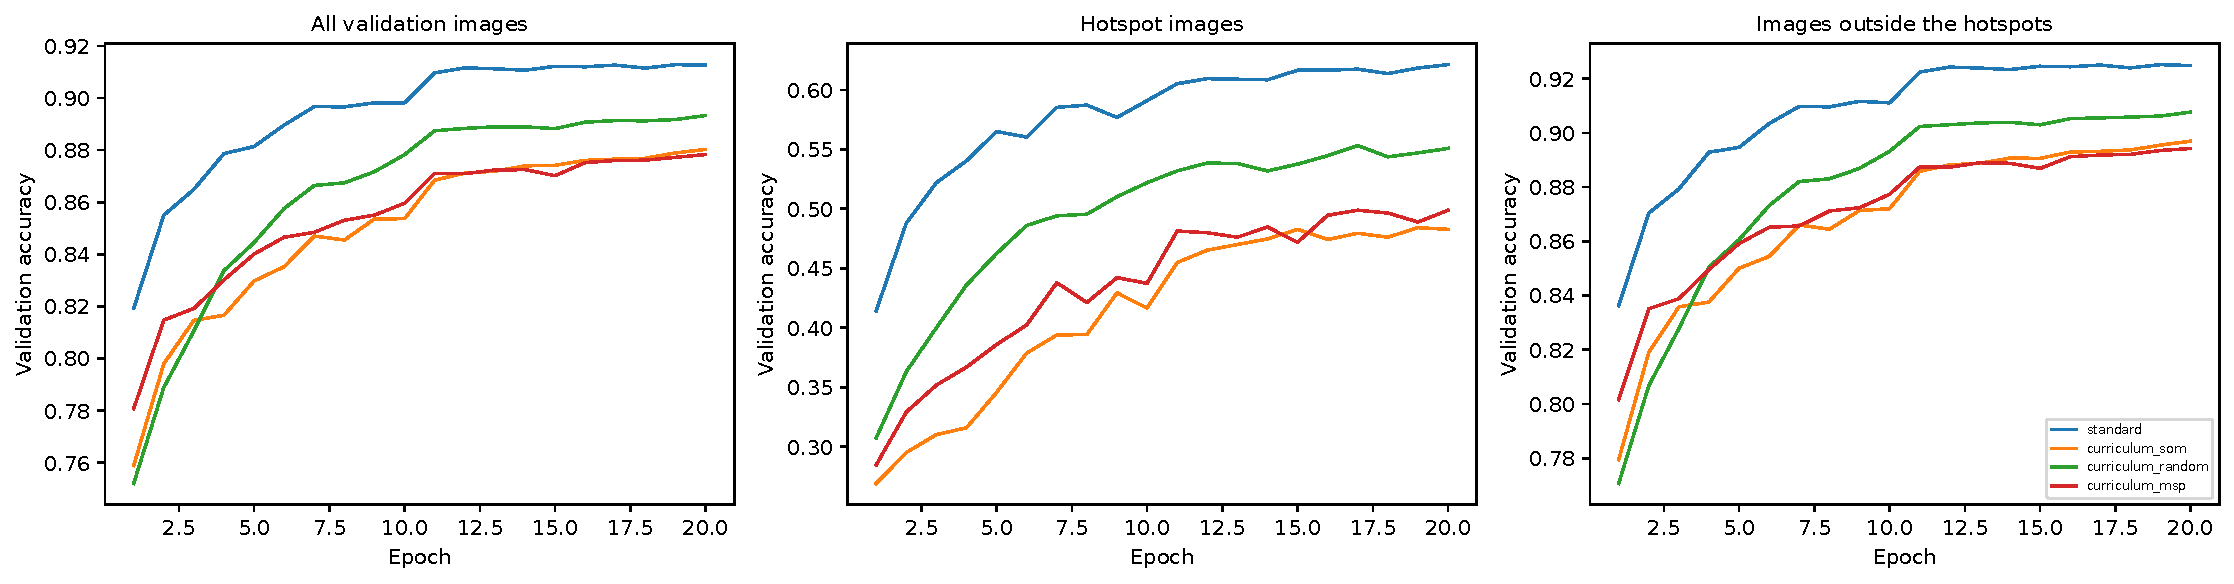
\includegraphics[width=\textwidth]{fig/hard_example_mining/curriculum_comparison/validation_accuracy_by_epoch.pdf}
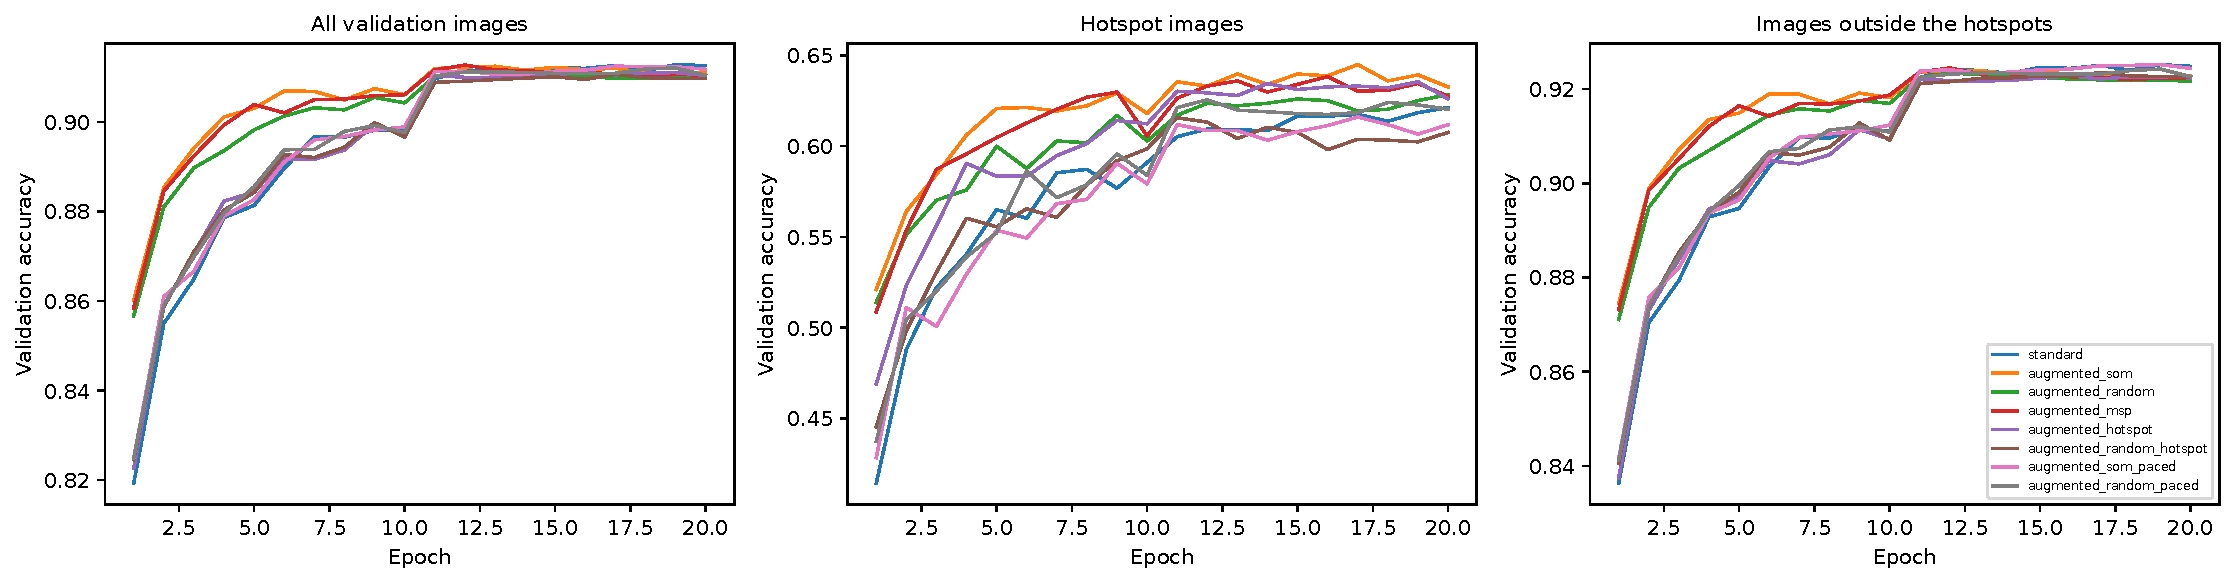
\includegraphics[width=\textwidth]{fig/targeted_augmentation/augmentation_comparison/validation_accuracy_by_epoch.pdf}
\caption{Validation accuracy per epoch (mean of 5 seeds) for the curriculum arms (top) and the augmentation arms (bottom): all images, hotspot images, and images outside the hotspots. The curriculum arms are behind \texttt{standard} from the first epoch and never catch up. The augmentation arms that add all copies at once rise faster in the first epochs (they see more images per epoch), and all arms end at about the same level.}
\label{fig:curves}
\end{figure}

\section{Re-analysis: new SOMs after retraining}\label{sec:reanalysis}

Table~\ref{tab:reanalysis} gives all measures and Figures~\ref{fig:reanalysis_measures} and~\ref{fig:reanalysis_purity} show the spread over seeds and example maps. One of the five statements holds (R4) and four do not (R1, R2, R3, R5).

\begin{table}[H]
\centering
\renewcommand{\arraystretch}{1.12}
\footnotesize
{\setlength{\tabcolsep}{3pt}\begin{tabular}{|>{\raggedright\arraybackslash}p{0.17\textwidth}|C{0.08\textwidth}|C{0.085\textwidth}|C{0.09\textwidth}|C{0.095\textwidth}|C{0.18\textwidth}|C{0.18\textwidth}|}
\hline
\textbf{Measure (validation)} & \textbf{Phase 2 map} & \textbf{standard} & \textbf{augm.\ som} & \textbf{augm.\ random} & \textbf{augm.\ som $-$ standard} & \textbf{augm.\ som $-$ augm.\ random} \\ \hline
Weighted purity (R1, R3) & 0.8933 & 0.8835 & 0.8748 & 0.8796 & $-$0.0087 [$-$0.0182, +0.0008] & $-$0.0048 [$-$0.0125, +0.0029] \\ \hline
Share of images in neurons with purity $<0.95$ & 0.4457 & 0.4344 & 0.4624 & 0.4519 & \textbf{+0.0281 [+0.0082, +0.0480]} & +0.0105 [$-$0.0068, +0.0278] \\ \hline
Class scatter index & 1.70 & 1.70 & 1.68 & 1.52 & $-$0.02 [$-$0.34, +0.30] & +0.16 [$-$0.14, +0.46] \\ \hline
Topographic error, \% (R5) & 5.37 & 6.02 & 6.83 & 6.98 & +0.81 [$-$0.16, +1.79] & $-$0.15 [$-$0.89, +0.59] \\ \hline
Hotspot error rate (R2, R4) & 0.4090 & 0.4062 & 0.4053 & 0.4372 & $-$0.0009 [$-$0.0225, +0.0207] & \textbf{$-$0.0319 [$-$0.0516, $-$0.0122]} \\ \hline
Share of errors in hotspots & 0.1975 & 0.2050 & 0.1847 & 0.2037 & $-$0.0203 [$-$0.0561, +0.0156] & $-$0.0189 [$-$0.0619, +0.0240] \\ \hline
Overall validation error & 0.0834 & 0.0865 & 0.0867 & 0.0878 & +0.0002 [$-$0.0018, +0.0022] & $-$0.0011 [$-$0.0024, +0.0002] \\ \hline
\end{tabular}}
\caption{SOM re-analysis on the validation split. Columns 2 to 5 are means over the 5 CNN seeds (the Phase 2 map is a single map). The last two columns are the paired difference per seed, averaged, with its 95\% $t$-interval (4 degrees of freedom); bold means the interval excludes 0. Linear CKA between the networks' embeddings: 0.896 within standard, 0.850 within augmented\_som, 0.843 within augmented\_random, 0.867 between arms. Source: \texttt{som\_reanalysis\_som\_15x15\_nb11\_ep250\_s42/tables/}.}
\label{tab:reanalysis}
\end{table}

\begin{itemize}[leftmargin=1.4em, itemsep=2pt]
  \item \textbf{R1, not met.} Weighted purity of \texttt{augmented\_som} is, if anything, lower than \texttt{standard} ($-0.0087$, interval $-0.0182$ to $+0.0008$; lower in all 5 seeds). The class boundaries in the map did not become sharper.
  \item \textbf{R2, not met.} The hotspot error rate is the same as after normal training ($-0.0009$, interval $-0.0225$ to $+0.0207$).
  \item \textbf{R3, not met.} Against the random-image control the purity difference is $-0.0048$ ($-0.0125$ to $+0.0029$).
  \item \textbf{R4, met.} Against the random-image control the hotspot error rate is lower by 3.2 points ($-0.0319$, interval $-0.0516$ to $-0.0122$; lower in all 5 seeds). Table~\ref{tab:reanalysis} shows why: it is the random arm whose hotspots got worse (0.437), while \texttt{augmented\_som} stayed at the \texttt{standard} level (0.405 against 0.406).
  \item \textbf{R5, not met.} Topographic error rose by 0.81 points on average and was higher in all 5 seeds; the upper end of the interval (1.79) is above the 1.0 tolerance, so we cannot say the new maps are as well ordered as after normal training.
  \item \textbf{Also reported.} After SOM-guided augmentation a larger share of validation images sits in low-purity neurons ($+0.028$, the only other interval that excludes 0). The class scatter index, the share of errors in hotspots and the overall validation error show no clear change. CKA is lower within the augmented arms (0.850 and 0.843) than within \texttt{standard} (0.896): networks trained with altered copies differ more from each other than normally trained ones. The mean quantization error of the new maps is 0.863 (\texttt{standard}), 0.973 (\texttt{augmented\_som}), 0.965 (\texttt{augmented\_random}) and 0.983 (\texttt{augmented\_msp}), against 0.899 for the Phase 2 map; each map is trained on a different network's embeddings, so these values are not directly comparable. Every new map uses 220 to 225 of its 225 neurons, and its 11 hotspots hold on average 459, 416, 430 and 431 validation images (Phase 2 map: 423).
  \item \textbf{Secondary run: the least-confident arm.} As on MNIST, under the addendum \texttt{MSP\_ARM\_ADDENDUM.md} (run \texttt{som\_reanalysis\_msp\_arm\_som\_15x15\_nb11\_ep250\_s42}). The new maps of \texttt{augmented\_msp} have a hotspot error rate of 0.413 against 0.406 for \texttt{standard} ($+0.0065$, interval $-0.0313$ to $+0.0443$, S1 not met). \texttt{augmented\_som} is not clearly better than \texttt{augmented\_msp} on hotspot error ($-0.0074$, $-0.0564$ to $+0.0416$, S2 not met) or purity ($+0.0004$, $-0.0063$ to $+0.0072$, S3 not met). The \texttt{augmented\_msp} maps are less pure than the \texttt{standard} ones ($-0.0091$, $-0.0163$ to $-0.0019$). The \texttt{standard} and \texttt{augmented\_som} cells reproduced the primary run exactly.
\end{itemize}

\begin{figure}[H]
\centering
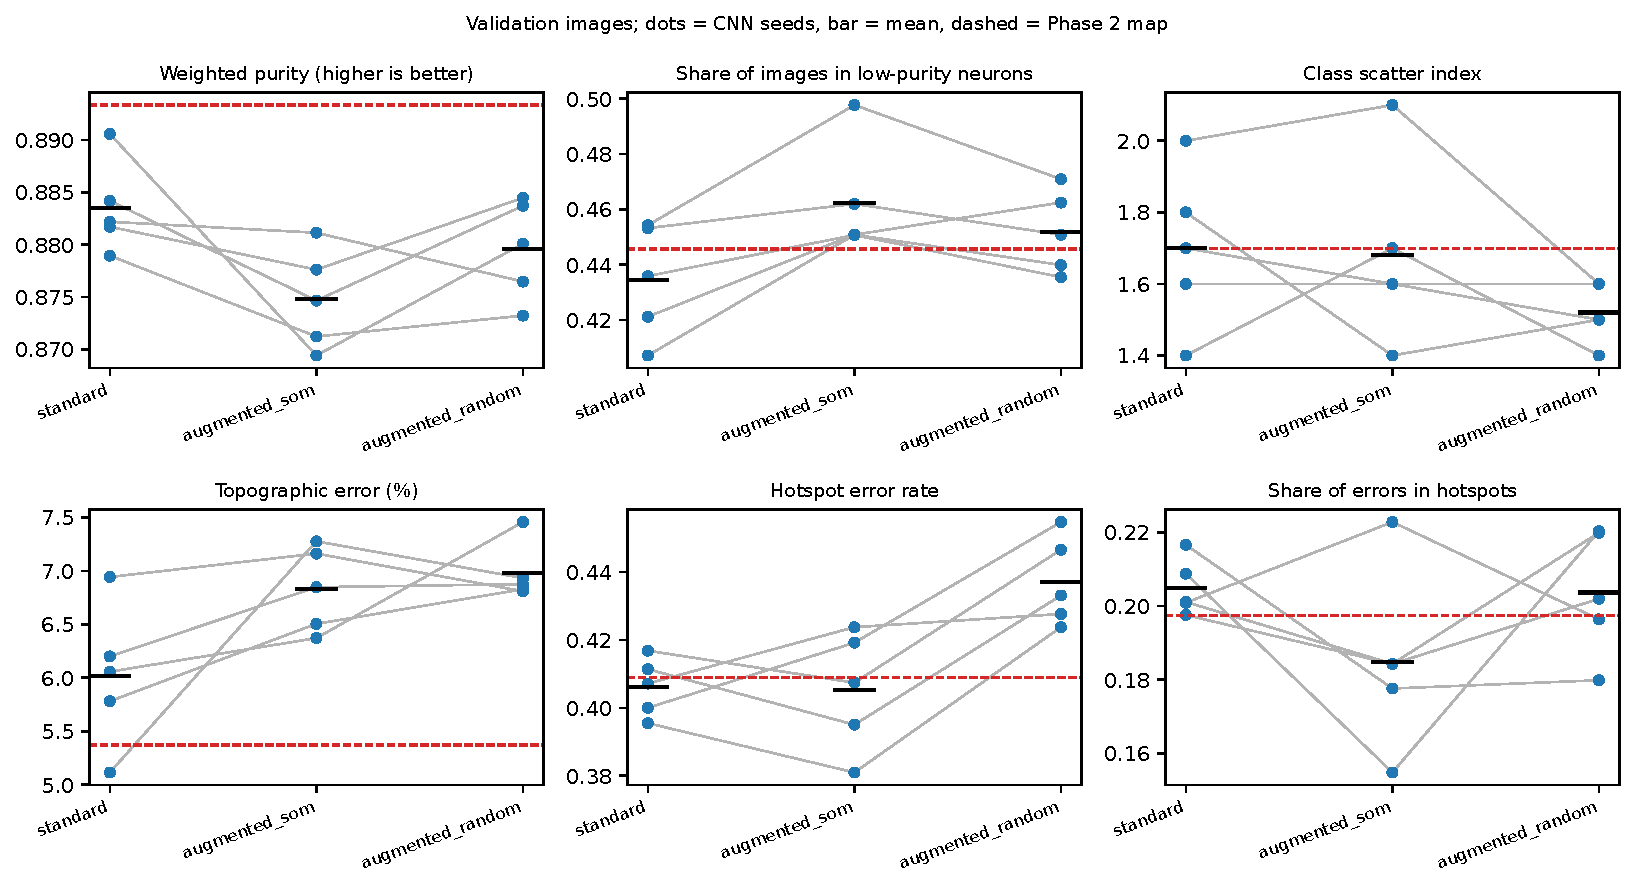
\includegraphics[width=\textwidth]{fig/som_reanalysis/map_measures_by_arm.pdf}
\caption{Map measures per arm on validation images. Each dot is one CNN seed (grey lines join the same seed), the black bar is the mean over seeds, and the dashed line is the Phase 2 map.}
\label{fig:reanalysis_measures}
\end{figure}

\begin{figure}[H]
\centering
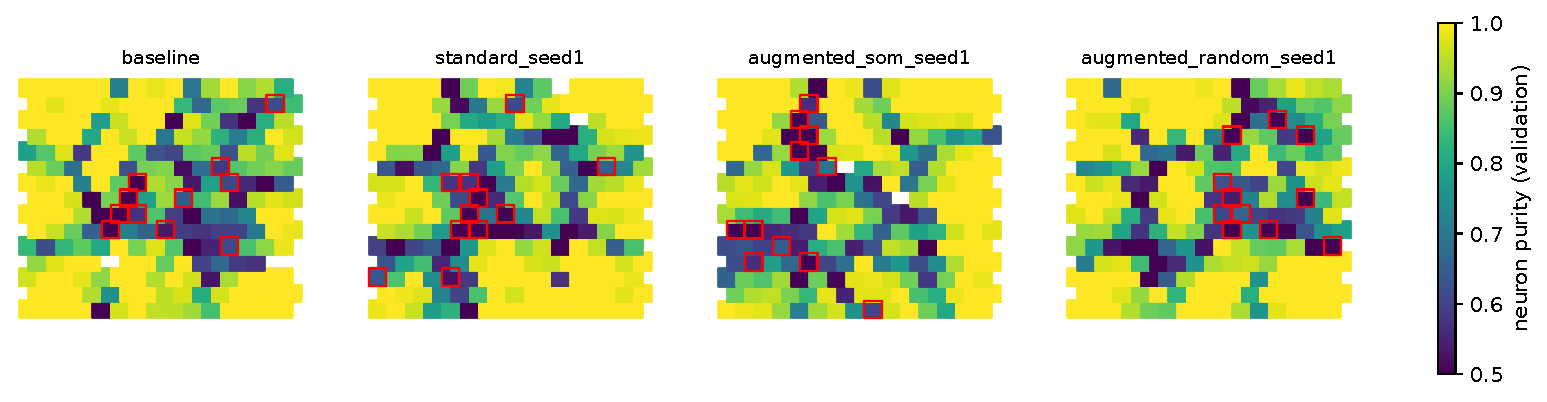
\includegraphics[width=\textwidth]{fig/som_reanalysis/purity_maps.pdf}
\caption{Neuron purity on validation images for the Phase 2 map and the three arms (seed 1). Red squares mark the hotspot neurons of each map. The hotspots are picked again for every map.}
\label{fig:reanalysis_purity}
\end{figure}

\textbf{How to read this.} The hotspots are the worst neurons of each map, chosen again for every map, so the hotspot error rate of a new map is not measured on the same images as before. Unlike on MNIST, the retrained \texttt{standard} networks have about the same hotspot error rate (0.406) as the Phase 2 map (0.409), but they are less pure (0.884 against 0.893) and less well ordered (6.0\% against 5.4\% topographic error), so the comparison between arms, not with the Phase 2 map, is the one to use. With 5 seeds and one SOM seed the intervals are wide, and a clear result for one comparison next to an unclear one should not be over-read. All of this is on Fashion-MNIST validation data.

\section{Errors fixed, and error per class (exploratory)}\label{sec:breakdown}

Both breakdowns are computed from the test predictions saved by the single test pass, as on MNIST: no network was retrained or re-run, and no criterion or threshold changed. They are descriptive, not success criteria.

\textbf{How many errors does retraining actually fix?} Table~\ref{tab:errors_fixed} gives counts. Normal training makes about 981 errors on the 10{,}500 test images, 152 of them on the 422 hotspot images. Retraining moves many individual errors: \texttt{augmented\_som} fixes about 335 of \texttt{standard}'s errors per seed and makes about 340 new ones, so the net change over all images is close to zero and varies from $-49$ to $+69$ between seeds. On the hotspot images \texttt{augmented\_som} has fewer errors than \texttt{standard} in 4 of the 5 seeds (about 8 fewer on average), but \texttt{augmented\_random} and \texttt{augmented\_msp} also have fewer in 3 and 4 seeds. Curriculum training adds 313 to 367 errors in every seed. The other arms are in the same table: the hotspot-only pool and its random control have more errors than \texttt{standard} overall in most seeds, \texttt{augmented\_som\_paced} has fewer hotspot errors in 4 of 5 seeds, and \texttt{curriculum\_random} and \texttt{curriculum\_msp} add 94 to 203 and 345 to 407 errors in every seed.

\begin{table}[H]
\centering
\renewcommand{\arraystretch}{1.1}
\footnotesize
{\setlength{\tabcolsep}{3pt}\begin{tabular}{|l|C{0.07\textwidth}|C{0.27\textwidth}|C{0.07\textwidth}|C{0.21\textwidth}|}
\hline
 & \multicolumn{2}{c|}{\textbf{All 10,500 test images}} & \multicolumn{2}{c|}{\textbf{422 hotspot test images}} \\ \hline
\textbf{Arm} & \textbf{Errors} & \textbf{Net fixed, per seed} & \textbf{Errors} & \textbf{Net fixed, per seed} \\ \hline
standard (CF1) & 980.6 & -- & 151.8 & -- \\ \hline
augmented\_som & 985.2 & $-33, +69, +15, -49, -25$ & 143.4 & $+4, +7, +19, -2, +14$ \\ \hline
augmented\_random & 987.4 & $-5, -17, +17, -34, +5$ & 147.8 & $+5, -3, +16, -4, +6$ \\ \hline
augmented\_msp & 990.2 & $-32, +46, +9, -39, -32$ & 148.6 & $-8, +16, +2, +1, +5$ \\ \hline
augmented\_hotspot & 995.0 & $-22, +20, -30, -37, -3$ & 153.4 & $-8, +6, -8, -12, +14$ \\ \hline
augmented\_random\_hotspot & 994.6 & $-46, -2, -14, +13, -21$ & 154.6 & $-17, -2, -2, +9, -2$ \\ \hline
augmented\_som\_paced & 982.0 & $-28, +10, +8, +4, -1$ & 147.8 & $-4, +7, +6, +5, +6$ \\ \hline
augmented\_random\_paced & 987.0 & $-18, +4, +7, -10, -15$ & 154.0 & $-4, -6, +0, +1, -2$ \\ \hline
curriculum\_som & 1326.0 & $-366, -313, -337, -367, -344$ & 218.8 & $-90, -54, -70, -69, -52$ \\ \hline
curriculum\_random & 1139.0 & $-203, -166, -94, -188, -141$ & 177.6 & $-39, -23, -16, -28, -23$ \\ \hline
curriculum\_msp & 1357.4 & $-379, -391, -345, -407, -362$ & 211.0 & $-67, -49, -54, -62, -64$ \\ \hline
\end{tabular}}
\caption{Test errors as counts (mean over the 5 seeds) and the net number of standard's errors each arm removed, per seed (seeds 1 to 5; positive means fewer errors than \texttt{standard} with the same seed). Net fixed = errors of \texttt{standard} that the arm gets right, minus new errors the arm makes. Exploratory; all arms are in the \texttt{tables/test\_errors\_fixed.csv} files of the two comparison runs.}
\label{tab:errors_fixed}
\end{table}

\textbf{Is the gain only on the SOM's own cells?} Hotspot error favours SOM-guided arms, because the SOM defines the hotspots. Classes are defined by no arm, so Table~\ref{tab:per_class} gives error per class. Here, unlike on MNIST, augmentation clearly moves errors between classes. Against \texttt{standard}, \texttt{augmented\_som} has lower error on Shirt ($-2.30$ points, interval $-3.54$ to $-1.03$), the class with the most errors, but higher error on T-shirt/top ($+1.33$), Dress ($+0.91$) and Bag ($+0.97$); all four intervals exclude 0. Against its controls, 5 of the 20 per-class intervals exclude 0: it is better than \texttt{augmented\_random} on Trouser and Coat and worse on Pullover, and better than \texttt{augmented\_msp} on Shirt and worse on T-shirt/top. With 30 intervals about 1 or 2 would exclude 0 by chance, so 9 is more than chance: SOM-guided copies, which are mostly upper-body clothing (Table~\ref{tab:pools}), mainly shift the Shirt/T-shirt boundary, with little net gain. The curriculum rows show where its loss comes from: \texttt{curriculum\_som} has higher error than \texttt{standard} on all 10 classes, most on Shirt (+11.8 points), Pullover (+6.2) and T-shirt/top (+5.9).

\begin{table}[H]
\centering
\renewcommand{\arraystretch}{1.1}
\footnotesize
{\setlength{\tabcolsep}{3pt}\begin{tabular}{|l|c|c|c|c|c|c|c|c|c|c|}
\hline
\textbf{Arm} & \textbf{T-shirt} & \textbf{Trouser} & \textbf{Pullover} & \textbf{Dress} & \textbf{Coat} & \textbf{Sandal} & \textbf{Shirt} & \textbf{Sneaker} & \textbf{Bag} & \textbf{Boot} \\ \hline
standard & 13.43 & 2.15 & 15.64 & 7.47 & 14.25 & 2.69 & 28.74 & 3.45 & 1.70 & 3.89 \\ \hline
augmented\_som & 14.76 & 1.89 & 15.45 & 8.38 & 14.04 & 2.50 & 26.44 & 3.87 & 2.67 & 3.85 \\ \hline
augmented\_random & 15.09 & 2.30 & 14.04 & 8.08 & 14.93 & 2.57 & 27.01 & 3.68 & 2.27 & 4.08 \\ \hline
augmented\_msp & 13.60 & 1.85 & 15.52 & 8.25 & 13.30 & 2.67 & 28.61 & 4.32 & 2.53 & 3.66 \\ \hline
curriculum\_som & 19.31 & 2.99 & 21.85 & 10.13 & 17.73 & 2.84 & 40.55 & 4.27 & 2.21 & 4.40 \\ \hline
curriculum\_random & 13.90 & 1.94 & 17.94 & 7.43 & 18.59 & 2.53 & 35.94 & 4.17 & 2.08 & 3.94 \\ \hline
curriculum\_msp & 20.15 & 2.82 & 20.65 & 8.88 & 18.04 & 3.01 & 44.97 & 4.44 & 1.87 & 4.46 \\ \hline
\end{tabular}}
\caption{Test error (\%) per class, mean over 5 seeds. Each class has 1,050 test images, so 0.1 points is about one image. Exploratory; paired intervals for every comparison are in the \texttt{test\_per\_class\_comparisons.csv} file of the augmentation run.}
\label{tab:per_class}
\end{table}

\section{Novelty detection after retraining}\label{sec:novelty_after}

Phase 3 showed that the SOM's quantization error (QE) separates SVHN house-number photographs \parencite{netzer2011reading} from Fashion-MNIST, but weakly (AUROC 0.789). Here we ask whether that still holds after retraining, and whether SOM-guided retraining changes it. We repeat the Phase 3 test on each of the 15 retrained networks (\texttt{standard}, \texttt{augmented\_som} and \texttt{augmented\_random}, 5 seeds each), each with the new SOM from Section~\ref{sec:reanalysis}. Fashion-MNIST validation images are the normal set and the 26{,}032 SVHN test images the novel set. Each network is also scored with max-softmax \parencite{hendrycks2017baseline}, energy \parencite{liu2020energy} and Mahalanobis distance \parencite{lee2018mahalanobis}, the last with a shrinkage covariance \parencite{ledoit2004wellconditioned}. Everything is fitted on training images only, and the Fashion-MNIST test split is not read. The statements, the margin of 0.01 AUROC and the rule that a result can be ``inconclusive'' \parencite{walker2011noninferiority} are the MNIST ones, unchanged.

As a check of the code, the Phase 1 network reproduces the Phase 3 results exactly (QE AUROC 0.789, max-softmax 0.884, energy 0.982, Mahalanobis 0.713).

\begin{table}[H]
\centering
\renewcommand{\arraystretch}{1.1}
\footnotesize
\begin{tabular}{|l|C{0.13\textwidth}|C{0.13\textwidth}|C{0.13\textwidth}|C{0.13\textwidth}|C{0.13\textwidth}|}
\hline
\textbf{Network} & \textbf{SOM QE} & \textbf{Max-softmax} & \textbf{Energy} & \textbf{Mahalanobis} & \textbf{Length only} \\ \hline
Phase 1 (reference) & 0.7894 & 0.8837 & 0.9821 & 0.7129 & 0.9949 \\ \hline
standard & 0.8378 (0.0941) & 0.8745 (0.0503) & 0.9715 (0.0151) & 0.7403 (0.0694) & 0.9845 (0.0090) \\ \hline
augmented\_som & 0.7149 (0.0760) & 0.8519 (0.0446) & 0.9462 (0.0377) & 0.5721 (0.0653) & 0.9484 (0.0403) \\ \hline
augmented\_random & 0.7438 (0.0910) & 0.8839 (0.0364) & 0.9596 (0.0225) & 0.6145 (0.0743) & 0.9551 (0.0275) \\ \hline
\end{tabular}
\caption{Novelty detection after retraining: AUROC for telling SVHN test images (novel) from Fashion-MNIST validation images (normal), mean (standard deviation) over 5 seeds. Each network is scored with its own new SOM. ``Length only'' is a check, not a detector: shorter embeddings are scored as more novel. Source: \texttt{novelty\_after\_retraining\_som\_15x15\_nb11\_ep250\_s42/results.json}.}
\label{tab:novelty_after}
\end{table}

\begin{table}[H]
\centering
\renewcommand{\arraystretch}{1.1}
\footnotesize
{\setlength{\tabcolsep}{4pt}\begin{tabular}{|l|C{0.11\textwidth}|C{0.13\textwidth}|C{0.20\textwidth}|C{0.13\textwidth}|C{0.13\textwidth}|}
\hline
\textbf{Network} & \textbf{QE AUPR} & \textbf{QE FPR@95} & \textbf{QE alarm: SVHN caught / normal flagged} & \textbf{Max-softmax FPR@95} & \textbf{Energy FPR@95} \\ \hline
Phase 1 (reference) & 0.825 & 0.420 & 0.030 / 0.051 & 0.307 & 0.063 \\ \hline
standard & 0.871 & 0.352 & 0.186 / 0.052 & 0.360 & 0.119 \\ \hline
augmented\_som & 0.781 & 0.533 & 0.021 / 0.051 & 0.441 & 0.246 \\ \hline
augmented\_random & 0.807 & 0.508 & 0.048 / 0.051 & 0.344 & 0.160 \\ \hline
\end{tabular}}
\caption{More measures from the same novelty run, mean over 5 seeds. AUPR treats SVHN as the positive class. FPR@95 is the share of normal images flagged when 95\% of SVHN is caught (lower is better). The QE alarm uses the threshold set from the training images (95th percentile of training QE). As in Phase 3, the QE alarm catches very little of SVHN on Fashion-MNIST, and after SOM-guided augmentation it catches less (2.1\%) than it wrongly flags among normal images (5.1\%). Source: \texttt{tables/cell\_scores.csv} of the novelty run.}
\label{tab:novelty_more}
\end{table}

\begin{itemize}[leftmargin=1.4em, itemsep=2pt]
  \item \textbf{N1: the SOM still detects novelty (shown).} In all 15 retrained networks the QE AUROC is above chance (0.593 to 0.935).
  \item \textbf{N2: SOM-guided retraining harms it (opposite shown).} The QE AUROC of \texttt{augmented\_som} is 0.123 lower than that of \texttt{standard} ($-0.151$ to $-0.094$), lower in all 5 seeds. The statement was that retraining does \emph{not} harm by more than the 0.01 margin; the interval lies entirely below $-0.01$, so the opposite is shown.
  \item \textbf{N3: against random augmentation, inconclusive.} The difference is $-0.029$, with a wide interval ($-0.179$ to $+0.121$).
  \item \textbf{N4: the gap to max-softmax widens (opposite shown).} QE minus max-softmax falls by 0.100 ($-0.165$ to $-0.035$) from \texttt{standard} to \texttt{augmented\_som}: SOM-guided retraining hurts QE more than it hurts max-softmax.
  \item \textbf{Energy stays best; Mahalanobis is weakest.} QE is within 0.01 AUROC of the best network-based score in none of the 15 networks. Energy, Mahalanobis and length also score lower after augmentation; max-softmax is lower only for \texttt{augmented\_som} (Table~\ref{tab:novelty_after}).
  \item \textbf{Single values move a lot.} The \texttt{standard} networks alone give QE AUROCs from 0.728 to 0.935; the Phase 1 network with SOM seeds 1 to 5 alone already gave 0.766 to 0.884 (Phase 3). This is why every comparison above is paired by seed.
  \item \textbf{Length explains less here than on MNIST.} Embedding length separates SVHN well in every network (AUROC 0.88 to 1.00), but QE follows length only weakly (mean Spearman correlation $-0.35$ for \texttt{standard}, $-0.02$ and $-0.08$ for the augmented arms; MNIST about $-0.9$), so the QE result is not just a length effect.
\end{itemize}

\section{What the results mean}\label{sec:meaning}

\textbf{How to read the tables.} In Table~\ref{tab:arms}, a higher accuracy and a lower error are better. In Table~\ref{tab:criteria}, the difference is ``first arm minus second arm'' in percentage points of error, so a \emph{negative} number means the first arm made fewer mistakes. If the interval in brackets does not include 0, the difference is probably real. Our test set has 10{,}500 images, so 0.1 points is about 11 images; the hotspots hold 422 test images, so one image is about 0.24 points.

\begin{itemize}[leftmargin=1.4em, itemsep=2pt]
  \item \textbf{Augmentation did not clearly fix hotspot mistakes (A1, A2 not met).} Normal training gets about 152 of the 422 hotspot images wrong; augmentation with SOM-chosen images gets about 143 wrong. That is 1.0 point better than random copies and 2.0 points better than normal training, but both intervals include 0. The failed primary criterion is the result; the criteria are not changed.
  \item \textbf{The rest of the images: no clear change, but damage cannot be ruled out (A3 not met).} The error outside the hotspots rose by 0.13 points on average, and the interval reaches 0.37 points, above the 0.2 limit.
  \item \textbf{The SOM was not better than ``least sure'' (E1).} Using the least-sure images (msp) gave a result that cannot be told apart from the SOM-chosen images, as on MNIST. The hotspot-only pool also could not be told apart from its random control (E3), and adding the copies gradually made no clear difference (E2; on MNIST it made things worse).
  \item \textbf{Curriculum learning lost to normal training (C1, C2 not met), more than on MNIST.} The curriculum CNNs made about 345 more mistakes out of 10{,}500 (+3.29 points), and the SOM-chosen order was worse than a random order. The learning curves (Figure~\ref{fig:curves}) show the curriculum arms behind from the first epochs, never catching up. A likely reason, which we did not test separately: the schedule lets in at most 40\% of the hard pool, so the hardest 60\% is never trained on. With the Fashion-MNIST pool at 41\% of the training set, that is about a quarter of all training images; on MNIST (pool 8.6\%) it was about 5\%.
  \item \textbf{The new maps: not cleaner, not better ordered.} SOM-guided augmentation kept the weak regions at the normal-training level while random augmentation made them worse (R4 met, R2 not met; on MNIST it was the other way round). The neurons are not purer (R1, R3), more images sit in mixed neurons, and the maps may be less well ordered (R5 not met).
  \item \textbf{Novelty detection got worse after SOM-guided retraining (N2, N4).} On MNIST retraining left it unchanged.
  \item \textbf{No sign of forgetting.} In every arm, the largest one-epoch fall in validation accuracy (mean over seeds) was 0.9 points or less (augmented\_hotspot was the largest), and every arm ended within 0.3 points of its best epoch.
\end{itemize}

\begin{table}[H]
\centering
\renewcommand{\arraystretch}{1.12}
\footnotesize
{\setlength{\tabcolsep}{3pt}\begin{tabular}{|>{\raggedright\arraybackslash}p{0.38\textwidth}|C{0.27\textwidth}|C{0.27\textwidth}|}
\hline
\textbf{Statement} & \textbf{Fashion-MNIST} & \textbf{MNIST} \\ \hline
A1 (primary): SOM copies beat random copies on hotspots & $-$1.04 [$-$3.22, +1.14], not met & $-$2.47 [$-$4.52, $-$0.68], met \\ \hline
A2: SOM copies beat normal training on hotspots & $-$1.99 [$-$4.79, +0.71], not met & $-$3.56 [$-$5.75, $-$1.37], met \\ \hline
A3: no damage outside hotspots (upper end $\le$ 0.2) & +0.13 [$-$0.12, +0.37], not met & $-$0.05 [$-$0.13, +0.02], met \\ \hline
C1: curriculum beats normal training & +3.29, worse & +0.45, worse \\ \hline
C2: SOM curriculum beats random curriculum & +9.76, worse & +9.18, worse \\ \hline
R2: new-map hotspots shrink vs standard & not met & met \\ \hline
R4: new-map hotspots shrink vs random & met & not met \\ \hline
R5: new map not less ordered & not met & met \\ \hline
N2: guided retraining does not harm novelty & opposite shown & inconclusive \\ \hline
\end{tabular}}
\caption{Fashion-MNIST next to MNIST. Differences in points of test error, first arm minus second, with the 95\% interval. R1 and R3 (purity) are not met on either dataset. MNIST values are from the MNIST Phase 4 report.}
\label{tab:mnist}
\end{table}

\textbf{What this means for the project overall.} All three steps of the loop ``SOM analysis $\rightarrow$ targeted retraining $\rightarrow$ new SOM structure'' were run on Fashion-MNIST with the MNIST design. The MNIST result does not carry over: on the harder dataset, adding altered copies of SOM-chosen images does not measurably reduce mistakes in the weak regions, does not change overall accuracy, does not make the new maps cleaner, and lowers the map's ability to flag novel images. Curriculum learning hurts on both datasets. Two conditions, both fixed before the test split was read, limit this test (Section~\ref{sec:deviation}): the copies had to be altered four times less than on MNIST, which leaves them less room to help, and the SOM pool covers 41\% of the training images, so it is far less selective than on MNIST and a random pool with the same class mix shares many of its images by chance. We therefore claim the SOM as a tool for \emph{finding and explaining} errors (Phase 2), not as a selector of training images.

\textbf{Limits.} 422 test images fall on hotspots, so the hotspot intervals are wide. The hotspots are defined by the SOM, so SOM-based arms have a built-in advantage on hotspot error. The pools come from one SOM, so they do not vary across seeds, and 5 seeds give limited power to separate small differences \parencite{bouthillier2021variance}. The design was copied from MNIST and not adapted to Fashion-MNIST (for example, the purity cut-off of 0.95 and the curriculum schedule).

\section{Deviation from the plan}\label{sec:deviation}

\begin{itemize}[leftmargin=1.4em, itemsep=2pt]
  \item \textbf{Smaller augmentation ranges (revision r3).} The MNIST ranges (rotation up to 10$^\circ$, shift up to 1 pixel, zoom 0.9 to 1.1, shear up to 8$^\circ$) failed the transform check made before any arm was trained: the Phase 1 network's validation accuracy fell from 91.66\% on the original images to 83.60\% on the altered ones, a drop of 8.1 points against a limit of 2. Fashion-MNIST items fill the 28$\times$28 frame, so zoom and rotation push sleeves and hems out of the image, and those are the parts that tell T-shirts, shirts, pullovers and coats apart. A rule was written down before the next check: halve all four ranges, and if that fails, halve once more, and if that fails, stop. Revision r2 (5$^\circ$, 0.5 pixel, 0.95 to 1.05, 4$^\circ$) gave 88.76\% (drop 2.9 points) and also failed; revision r3 (2.5$^\circ$, 0.25 pixel, 0.975 to 1.025, 2$^\circ$) gave 90.46\% (drop 1.2 points) and passed. Both failed checks are kept; all augmentation results above use r3. Examples of altered copies are in the Appendix.
  \item \textbf{Macro-F1 guard 0.0033.} Measured by the MNIST rule on the Fashion-MNIST \texttt{standard} arm; the MNIST value (0.0016) measures MNIST's seed-to-seed spread and was not reused.
  \item \textbf{Where the outcome is recorded.} The protocol says its outcome goes in its section 5, but writing there would break the SHA-256 stamp, so the outcome is in \texttt{RETRAINING\_RESULTS.md} next to it, as for MNIST.
\end{itemize}

All of these are recorded in \texttt{src/v1\_fashion\_mnist/docs/DEVIATIONS.md}. No criterion, threshold or test comparison was changed after the test split was used.

\section{Leakage Control}

\begin{itemize}[leftmargin=1.4em, itemsep=1pt]
  \item Pools, augmented copies and training use training images only. The transform check and the macro-F1 guard use validation images only.
  \item The 11 hotspots were chosen from validation errors; this is declared, and it is why the final judgement is made on the test split.
  \item Criteria, thresholds and the guard value were written down and stamped (SHA-256 of the protocol and the configuration, 2026-11-22 07:17 UTC) before the test split was opened. It was opened once, by the \texttt{final\_test} stage, and not re-run.
  \item The Fashion-MNIST protocol was written after the MNIST results were known; it copies MNIST's design instead of adapting it, and no Fashion-MNIST result existed when it was written.
  \item All arms use the same data, seeds and training recipe. Finished runs are never overwritten; each changed augmentation revision got a new run ID (\texttt{\_r2}, \texttt{\_r3}).
  \item The re-analysis, including the secondary run with the least-confident arm, uses training and validation images only; the test split was not read.
  \item The novelty test after retraining fits everything on training images, uses Fashion-MNIST validation and SVHN test images for scoring only, and does not read the Fashion-MNIST test split. Its statements and margin were fixed before the run, and the run records SHA-256 checks of its inputs.
\end{itemize}

\section{Limitations and future work}\label{sec:open}

All items of the Phase 4 plan are done. Three limits of the results are stated here.

\begin{itemize}[leftmargin=1.4em, itemsep=2pt]
  \item \textbf{Which arms were re-analysed.} The three arms of the SOM re-analysis were chosen on MNIST after its retraining results were known, and kept unchanged here; the least-confident arm is a secondary run, reported next to the primary statements, not in place of them.
  \item \textbf{A design made for MNIST.} The pool rule, the curriculum schedule and (before the transform check) the augmentation ranges were fixed on MNIST. On Fashion-MNIST the pool covers 41\% of the training images and the curriculum never shows most of it. A pool rule or schedule chosen for this dataset, on validation data and under a new protocol, could give a fairer test of SOM guidance.
  \item \textbf{Far novelty only.} The novelty test after retraining uses SVHN only. Phase 3 includes a near-novelty test with held-out clothing classes, but for the Phase 1 network only; repeating it on the retrained networks is future work.
\end{itemize}

\printbibliography[title={References}]

\clearpage
\appendix
\section{Further confusion matrices and examples}

Each figure shows CF1 (standard), CF2 of the named arm, and their difference, as in Figure~\ref{fig:cf_aug}.

\begin{figure}[H]
\centering
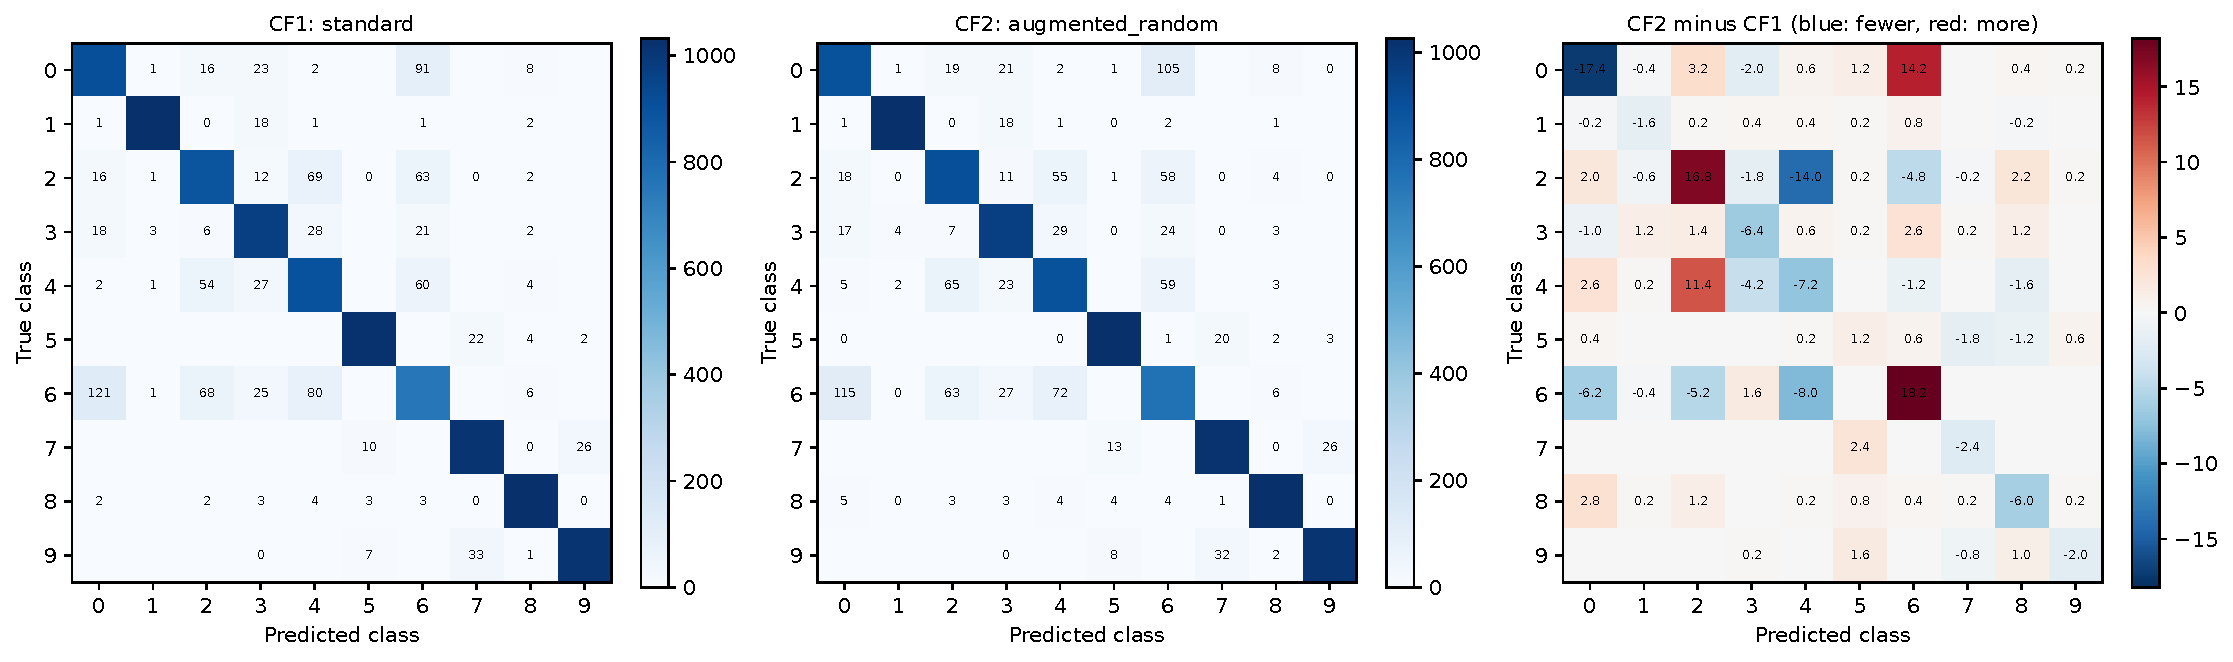
\includegraphics[width=\textwidth]{fig/targeted_augmentation/augmentation_comparison/confusion_standard_vs_augmented_random.pdf}\\[4pt]
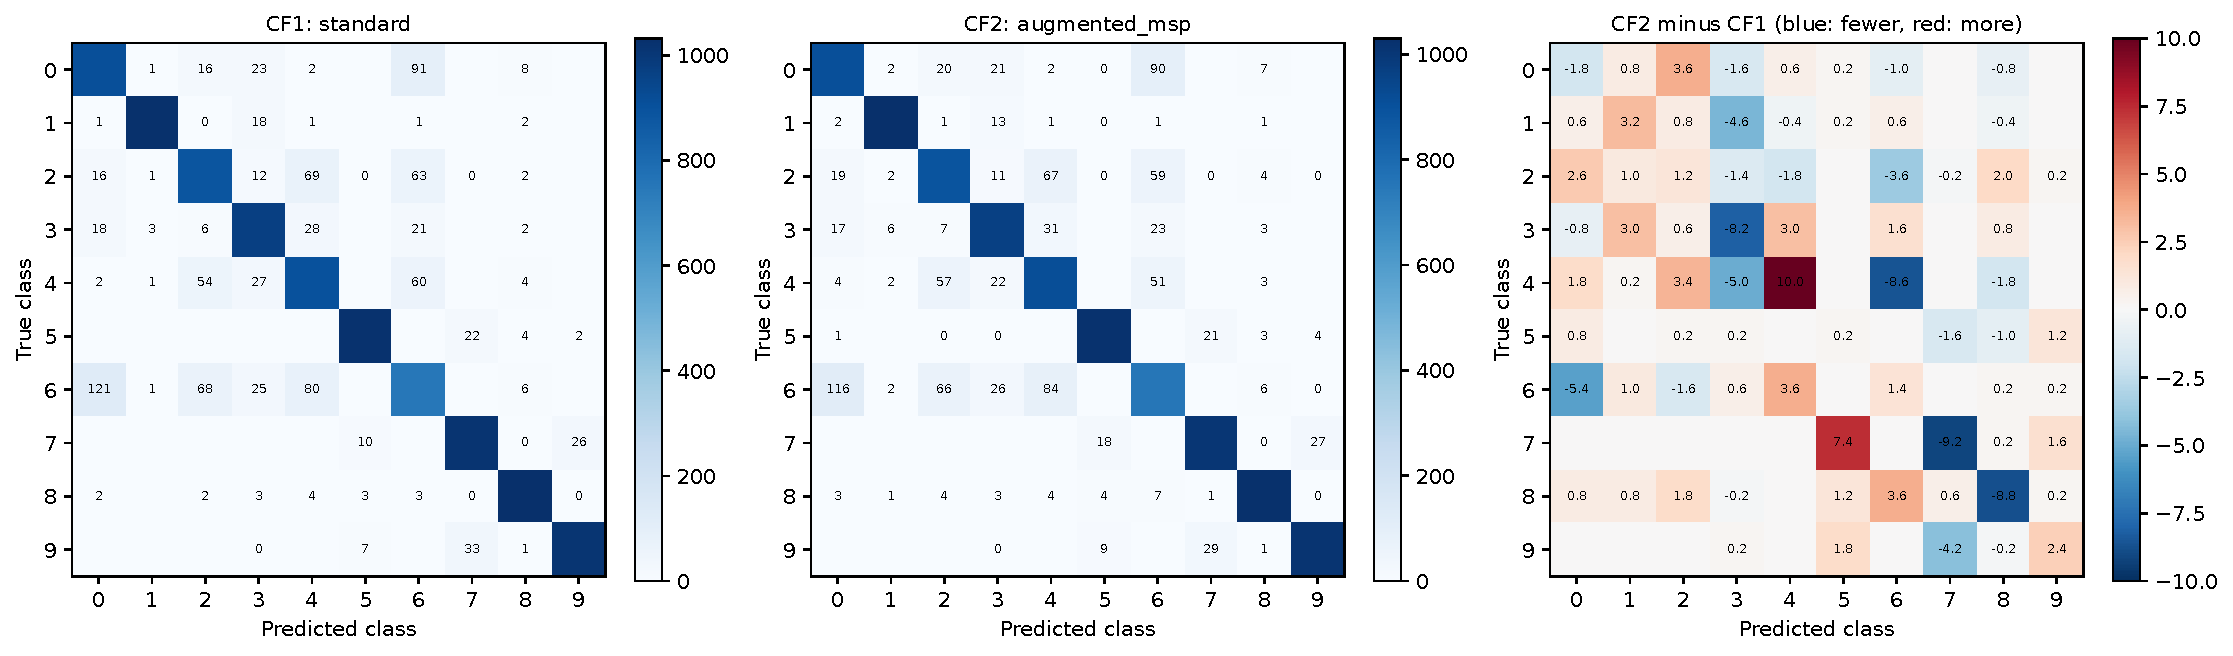
\includegraphics[width=\textwidth]{fig/targeted_augmentation/augmentation_comparison/confusion_standard_vs_augmented_msp.pdf}\\[4pt]
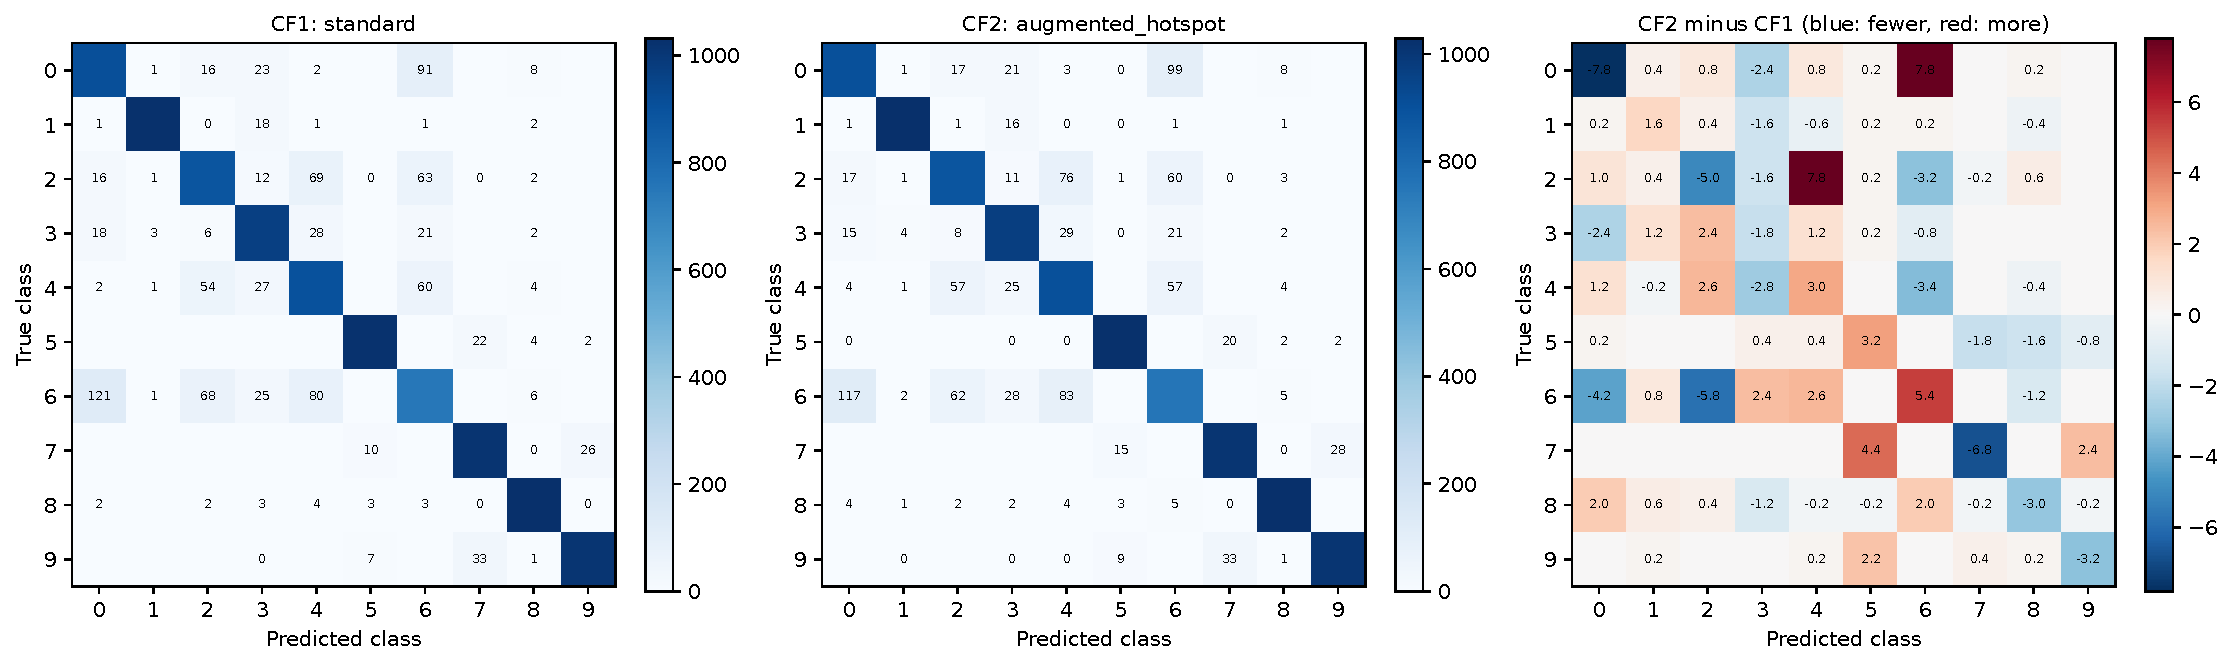
\includegraphics[width=\textwidth]{fig/targeted_augmentation/augmentation_comparison/confusion_standard_vs_augmented_hotspot.pdf}\\[4pt]
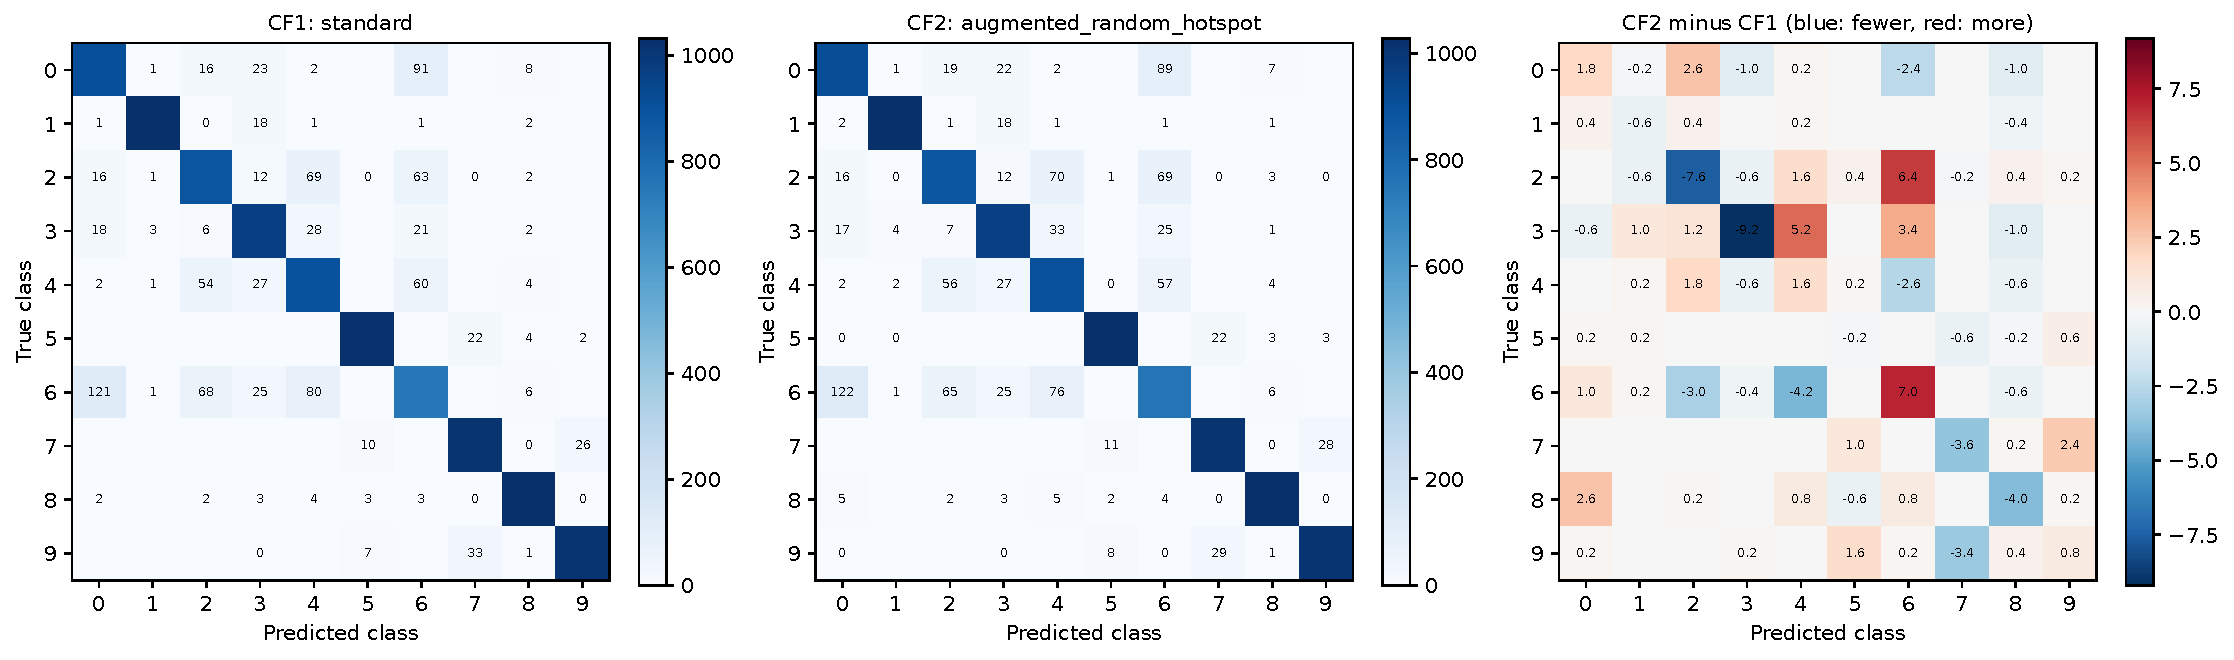
\includegraphics[width=\textwidth]{fig/targeted_augmentation/augmentation_comparison/confusion_standard_vs_augmented_random_hotspot.pdf}
\caption{CF2 of augmented\_random, augmented\_msp, augmented\_hotspot and augmented\_random\_hotspot (top to bottom).}
\end{figure}

\begin{figure}[H]
\centering
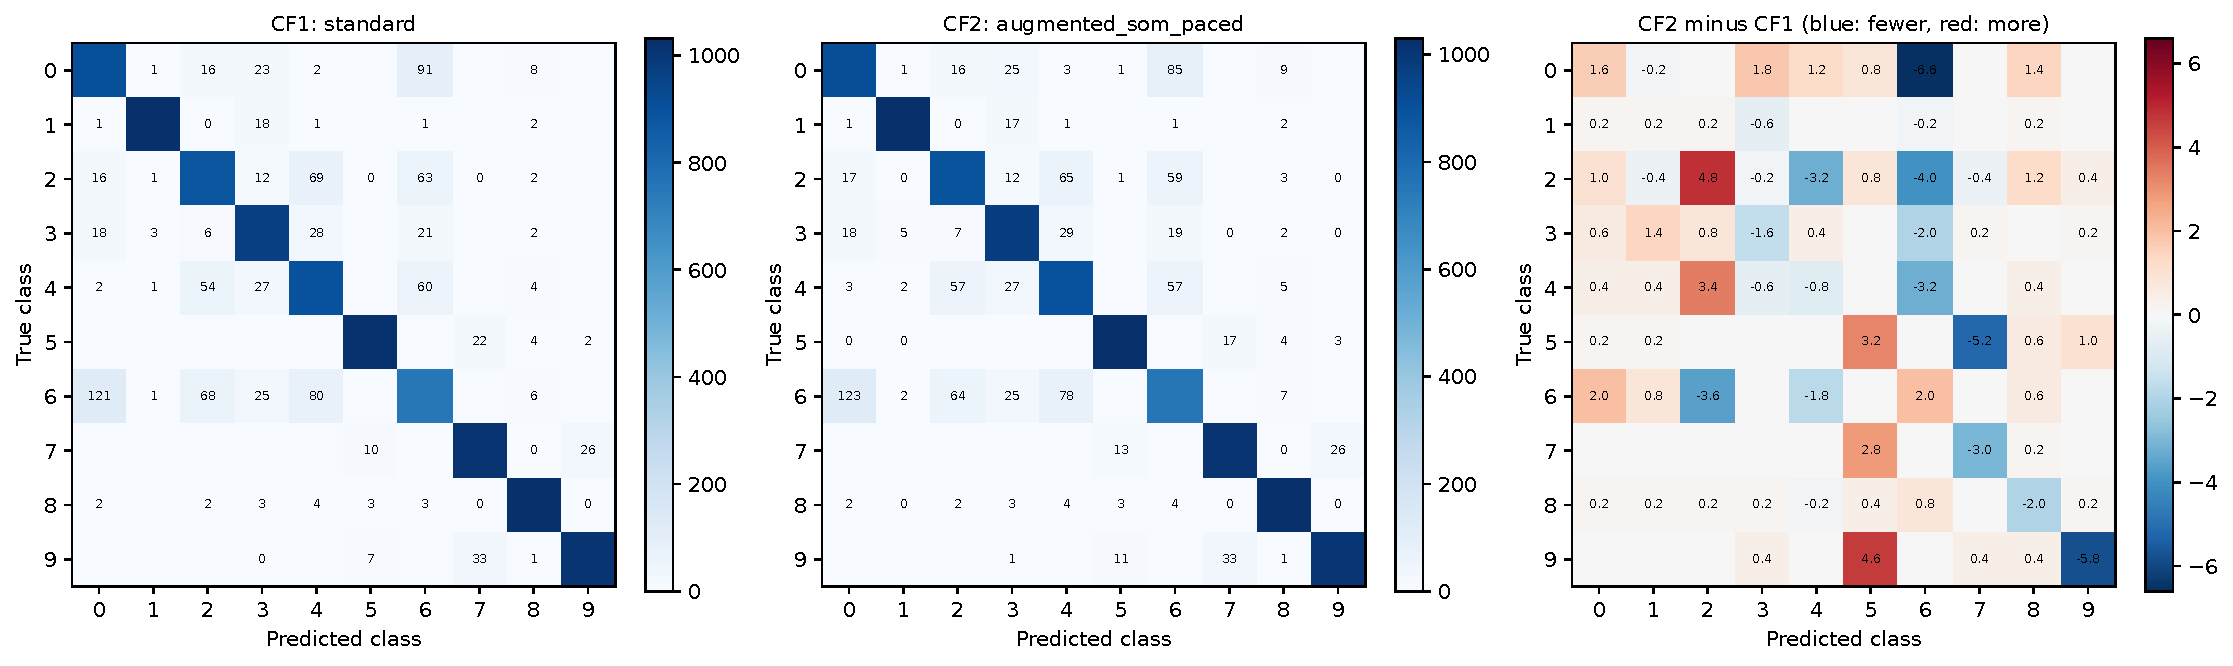
\includegraphics[width=\textwidth]{fig/targeted_augmentation/augmentation_comparison/confusion_standard_vs_augmented_som_paced.pdf}\\[4pt]
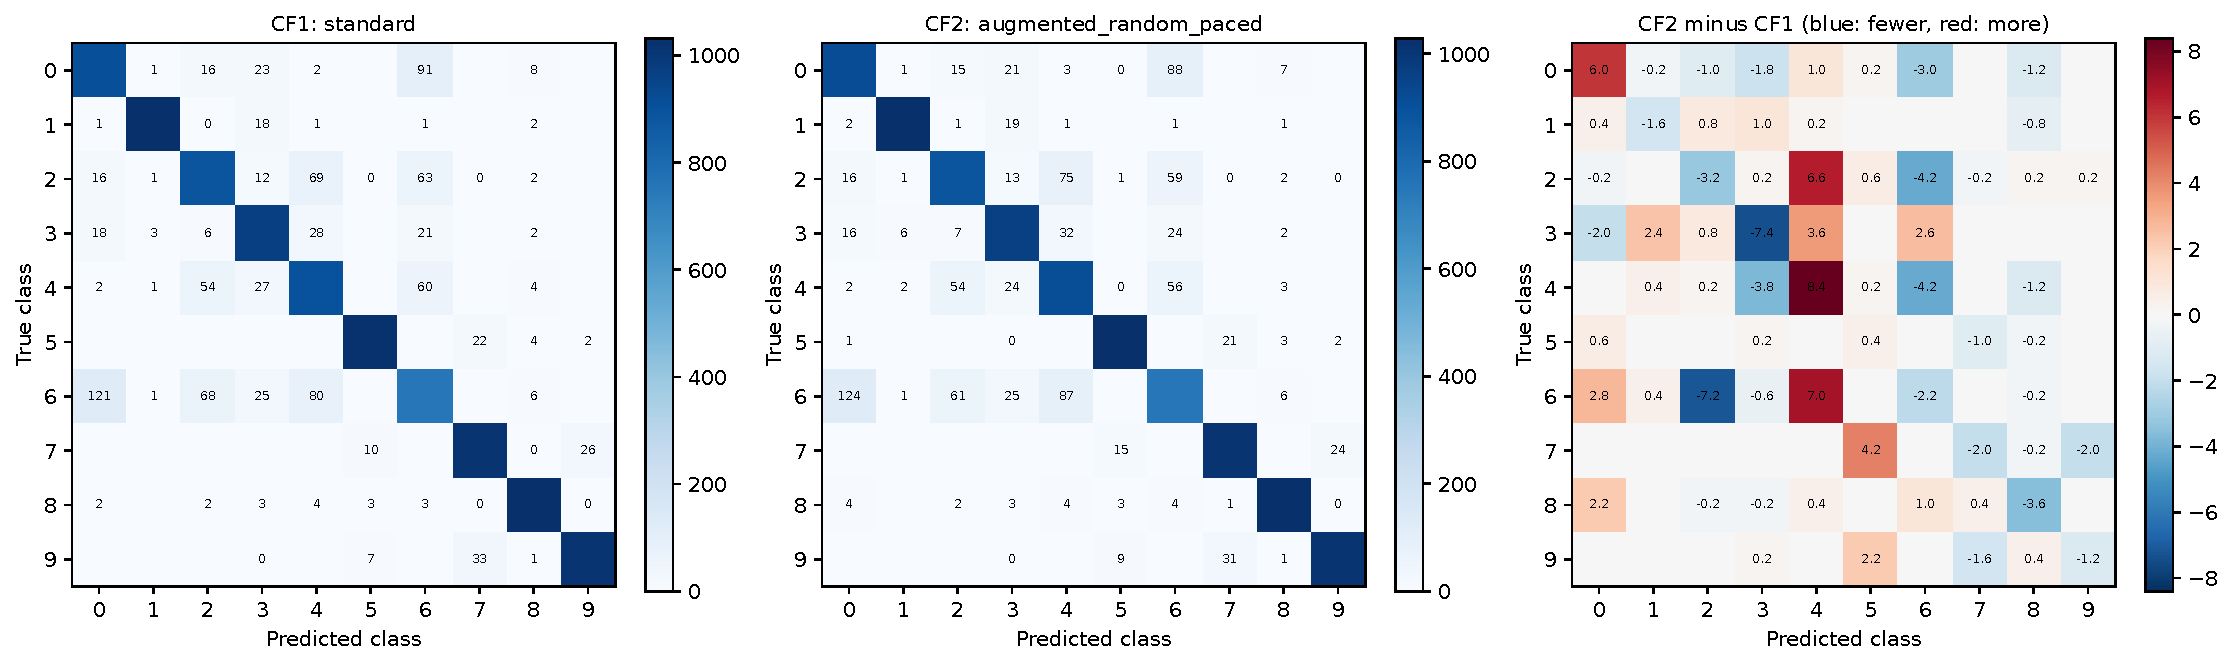
\includegraphics[width=\textwidth]{fig/targeted_augmentation/augmentation_comparison/confusion_standard_vs_augmented_random_paced.pdf}\\[4pt]
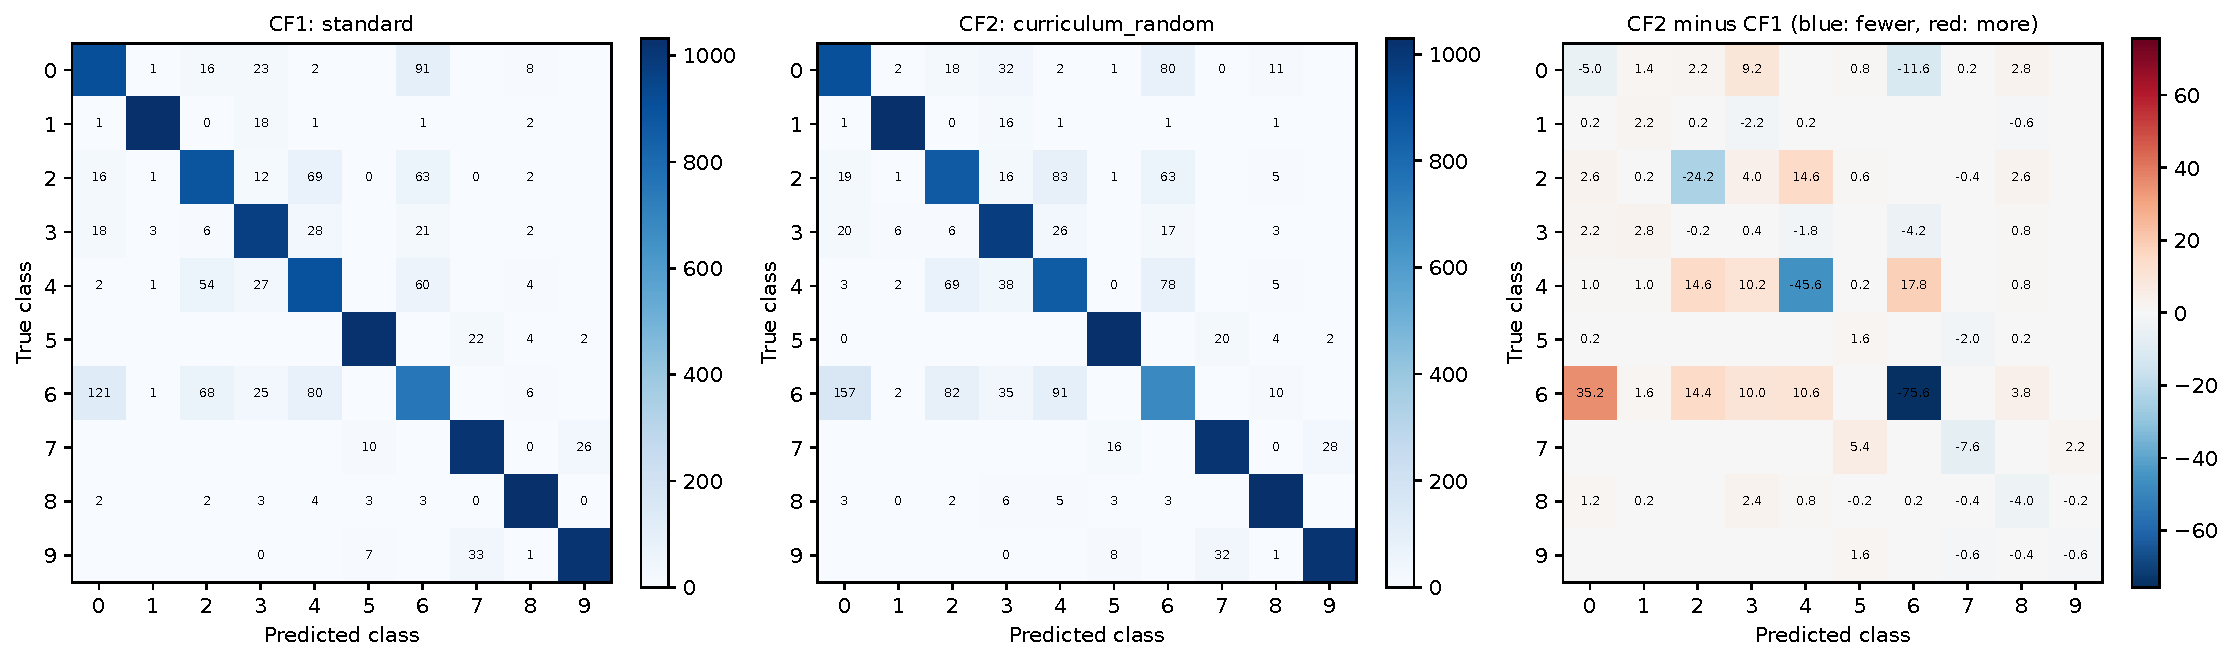
\includegraphics[width=\textwidth]{fig/hard_example_mining/curriculum_comparison/confusion_standard_vs_curriculum_random.pdf}\\[4pt]
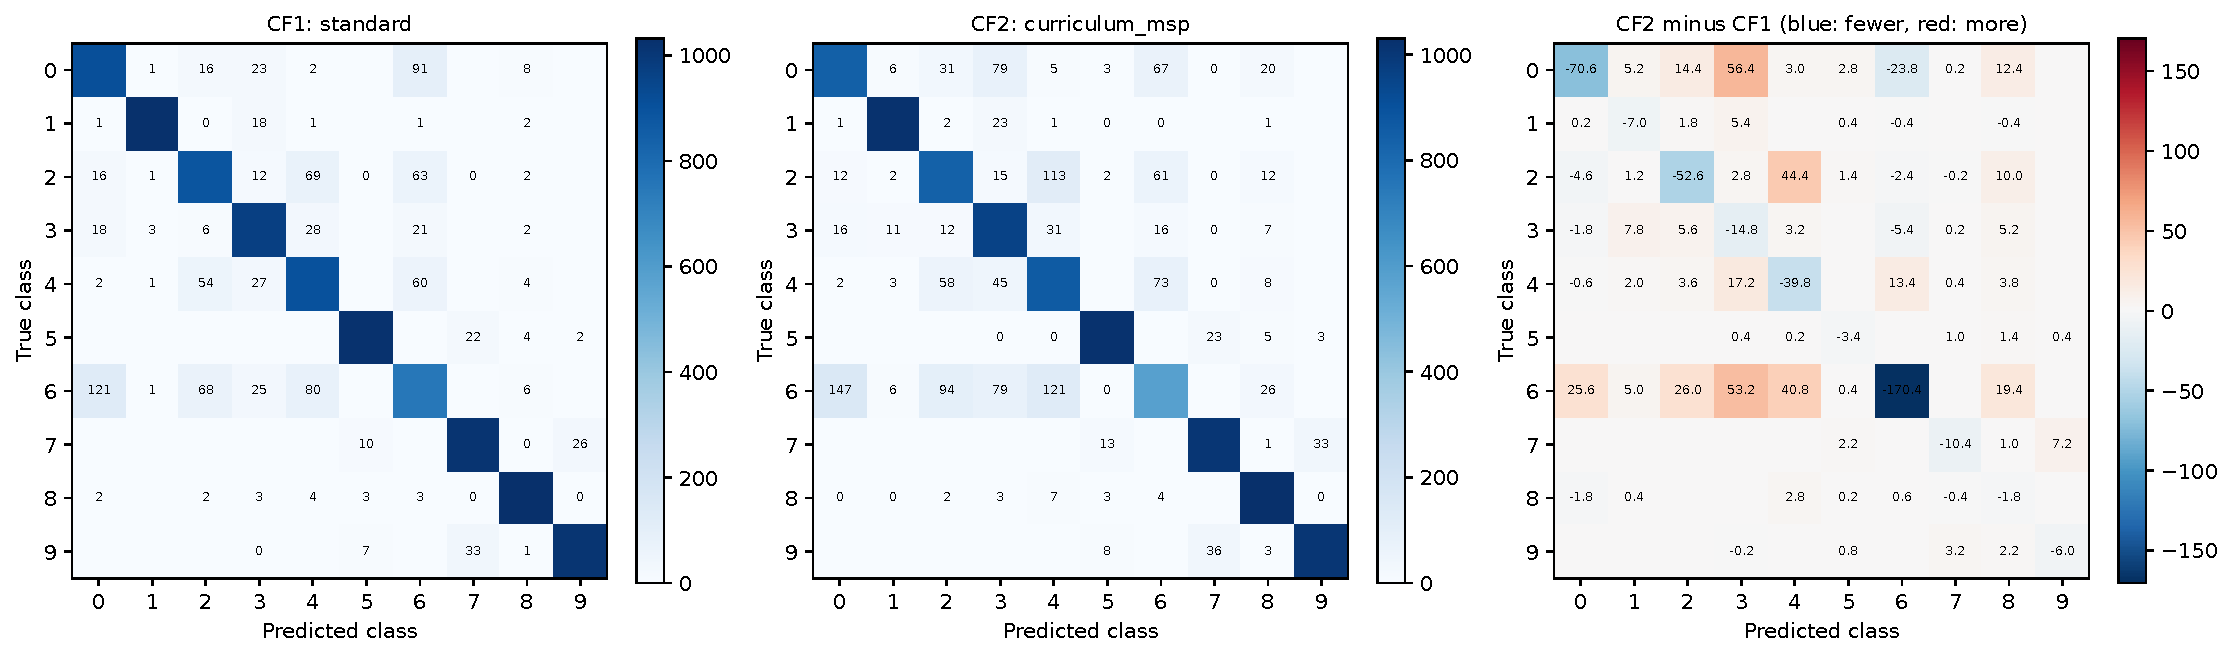
\includegraphics[width=\textwidth]{fig/hard_example_mining/curriculum_comparison/confusion_standard_vs_curriculum_msp.pdf}
\caption{CF2 of augmented\_som\_paced, augmented\_random\_paced, curriculum\_random and curriculum\_msp (top to bottom).}
\end{figure}

\begin{figure}[H]
\centering
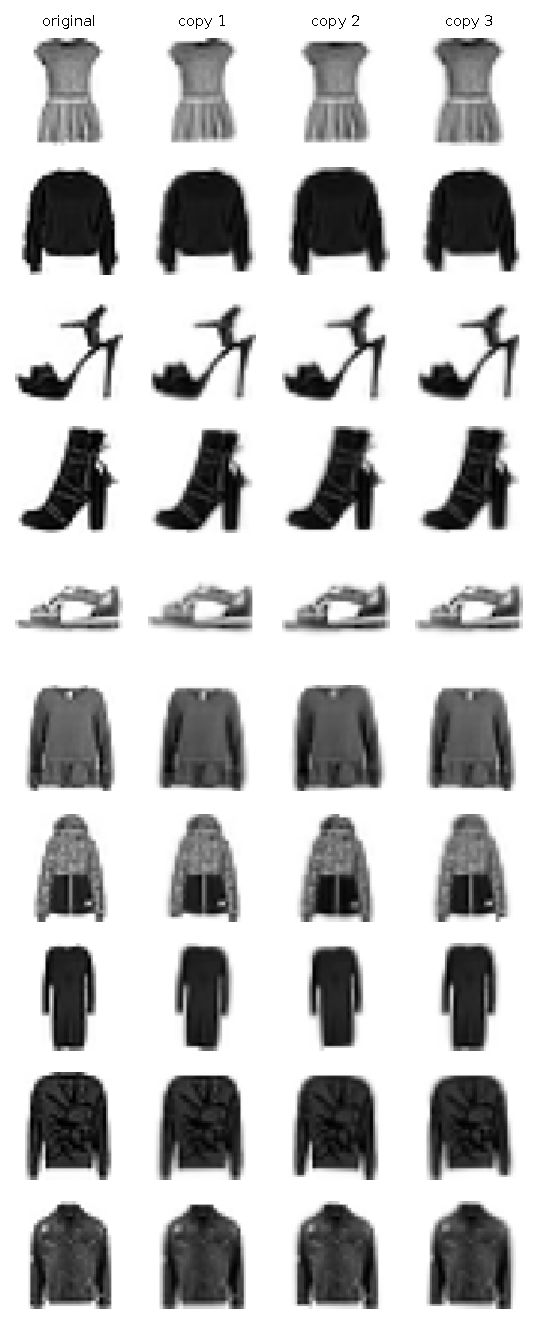
\includegraphics[height=0.55\textheight,keepaspectratio]{fig/targeted_augmentation/augmentation_comparison/augmentation_contact_sheet.pdf}
\caption{Ten training images from the hard pool (left column) and their three altered copies (revision r3: rotation up to 2.5$^\circ$, shift up to 0.25 pixel, zoom 0.975 to 1.025, shear up to 2$^\circ$).}
\end{figure}

\begin{figure}[H]
\centering
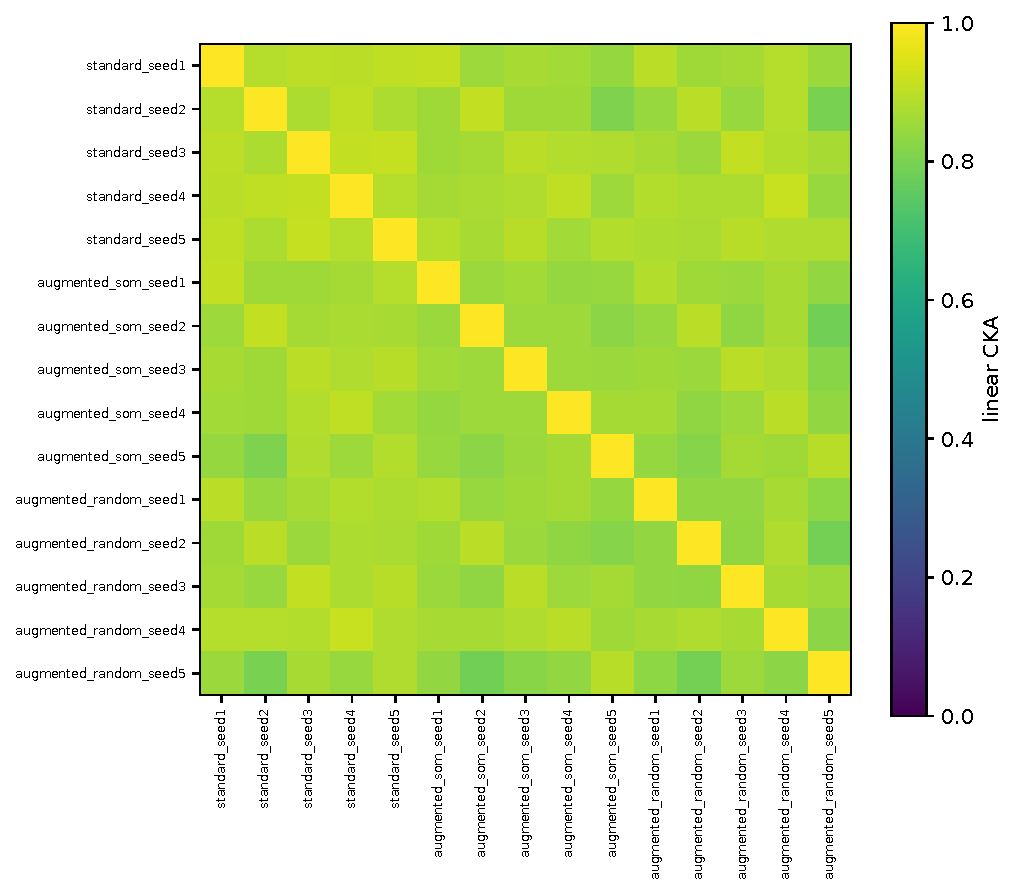
\includegraphics[width=\textwidth]{fig/som_reanalysis/embedding_similarity_cka.pdf}
\caption{Linear CKA between the embeddings of the 15 retrained networks (validation images).}
\end{figure}

\begin{figure}[H]
\centering
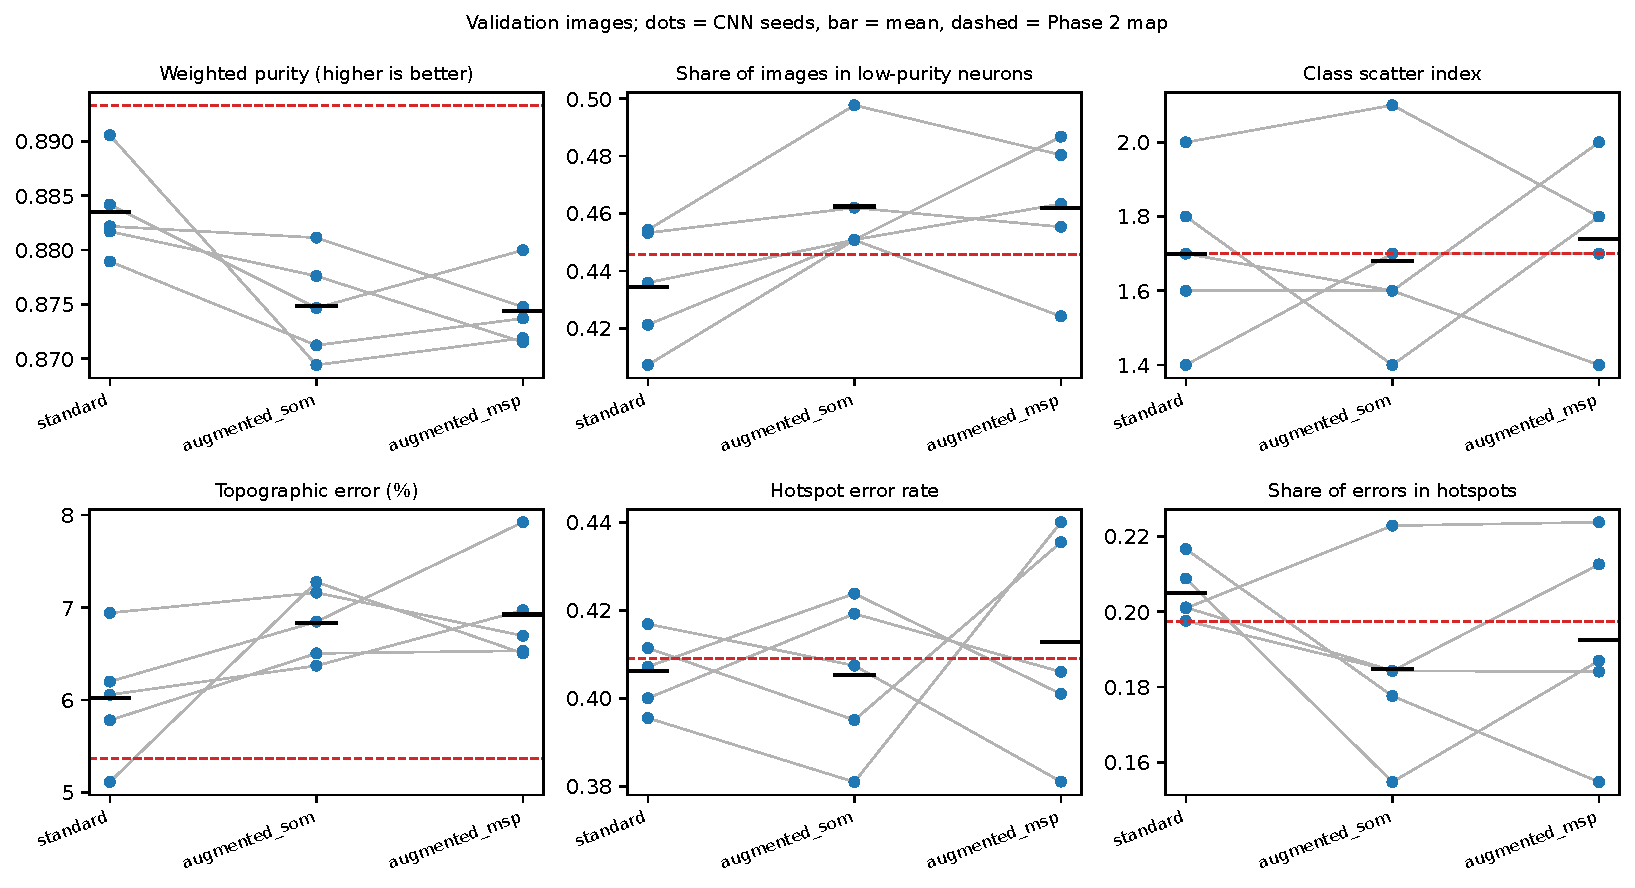
\includegraphics[width=\textwidth]{fig/som_reanalysis/msp_arm/map_measures_by_arm.pdf}\\[4pt]
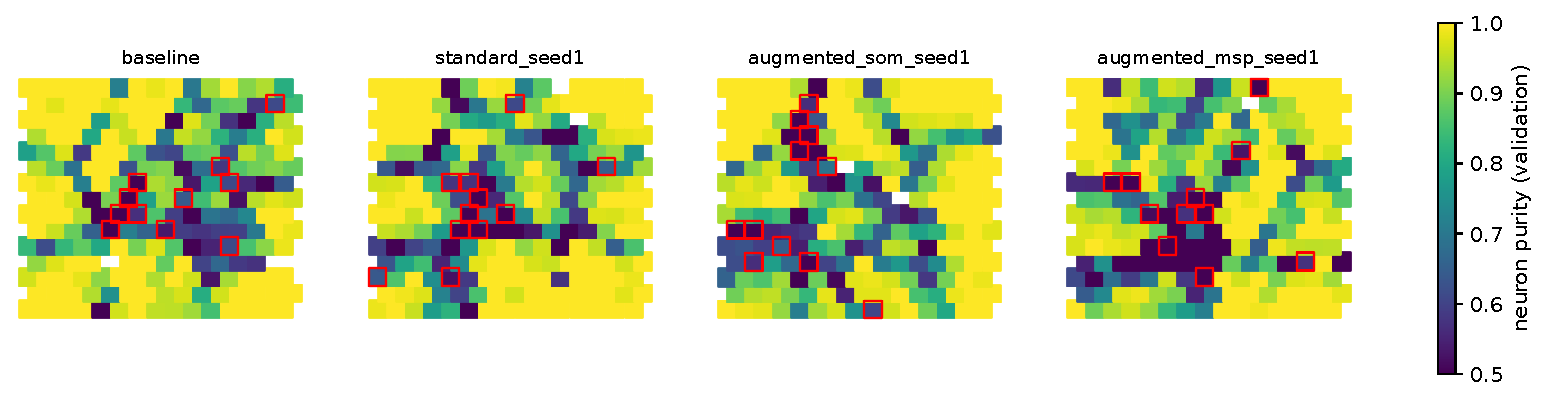
\includegraphics[width=\textwidth]{fig/som_reanalysis/msp_arm/purity_maps.pdf}
\caption{Secondary re-analysis run with the least-confident arm: map measures per arm (top, as in Figure~\ref{fig:reanalysis_measures}) and neuron purity maps, seed 1 (bottom, as in Figure~\ref{fig:reanalysis_purity}). As in the primary run, the least-confident arm's new maps are not purer than the \texttt{standard} ones.}
\end{figure}

\begin{figure}[H]
\centering
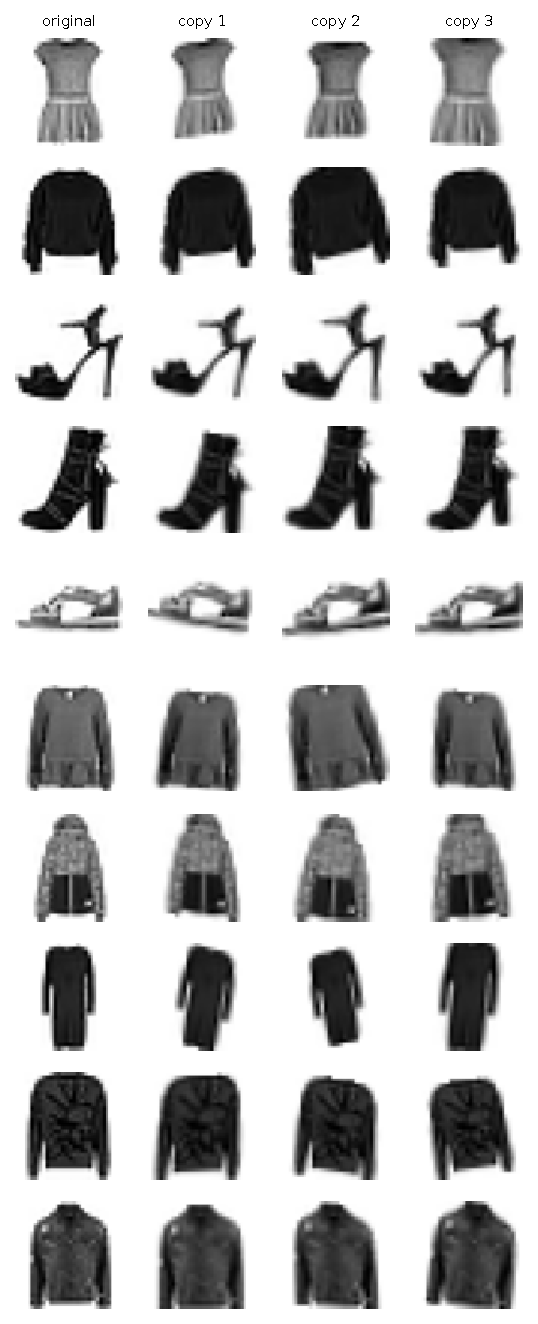
\includegraphics[height=0.5\textheight,keepaspectratio]{fig/targeted_augmentation/failed_checks/augmentation_contact_sheet_r1.pdf}
\caption{The MNIST augmentation ranges (revision r1: rotation up to 10$^\circ$, shift up to 1 pixel, zoom 0.9 to 1.1, shear up to 8$^\circ$), which failed the transform check (validation accuracy 91.66\% to 83.60\%). Kept as the record; no arm was trained with them.}
\end{figure}

\begin{figure}[H]
\centering
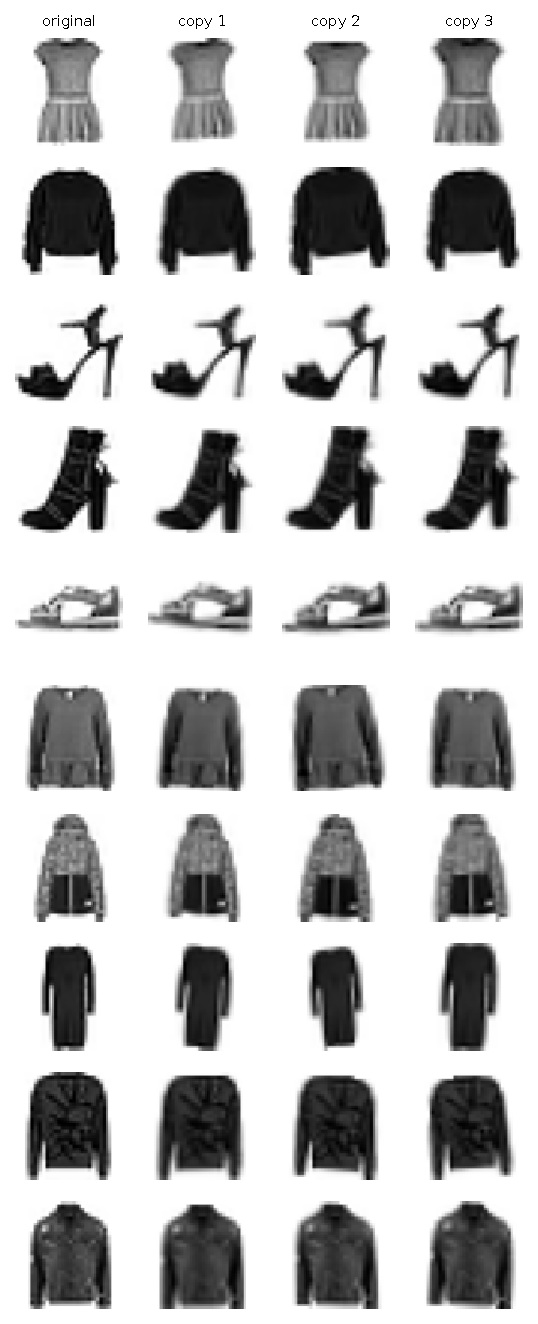
\includegraphics[height=0.5\textheight,keepaspectratio]{fig/targeted_augmentation/failed_checks/augmentation_contact_sheet_r2.pdf}
\caption{The halved ranges (revision r2: 5$^\circ$, 0.5 pixel, 0.95 to 1.05, 4$^\circ$), which also failed (91.66\% to 88.76\%). Kept as the record; no arm was trained with them.}
\end{figure}

\end{document}
